% !Mode:: "TeX:UTF-8"
\documentclass[master]{bnuthesis}
% \documentclass[%
%   bachelor|master|doctor, % mandatory option
%   xetex|pdftex|dvips|dvipdfm, % optional
%   openany|operight,  % 连续页面,或者右侧打开
%   secret,  % 是否涉密
%   arialtoc,arialtitle]{bnuthesis}

% 所有其它可能用到的包都统一放在这里,可以根据实际需要添加或者删除。
\usepackage{bnutils}
\usepackage{amsmath,bm}
\usepackage{mathtools}
\usepackage{threeparttable}
\usepackage{graphicx}
\usepackage{adjustbox}
\DeclarePairedDelimiter{\abs}{\lvert}{\rvert}
% 你可以在这里修改配置文件中的定义,导言区可以使用中文。
% \def\myname{薛瑞尼}

\begin{document}
% 定义所有的eps文件在figures子目录下
\graphicspath{{figures/}}

%%% 封面部分
\frontmatter
% !Mode:: "TeX:UTF-8"
%%% Local Variables:
%%% mode: latex
%%% TeX-master: t
%%% End:
%\secretlevel{绝密} \secretyear{10}

\ctitle{基于模糊不确定性和生成对抗网络的遥感影像弱监督学习分类}
%\makeatletter
%\cdegree{硕士}

\makeatother

\cauthor{江涛}
\csupervisor{余先川教授} %\\ \hspace*{6em}}
\cdepartment{信息科学与技术学院 2016级}
\cmajor{计算机软件与理论}
\cnum{201621210026}
\cdate{\the\year 年 \the\month 月}

\etitle{An Introduction to \LaTeX{} Thesis Template of Beijing Normal University}

% 定义中英文摘要和关键字
\begin{cabstract}
  论文的摘要是对论文研究内容和成果的高度概括。摘要应对论文所研究的问题及其研究目
  的进行描述,对研究方法和过程进行简单介绍,对研究成果和所得结论进行概括。摘要应
  具有独立性和自明性,其内容应包含与论文全文同等量的主要信息。使读者即使不阅读全
  文,通过摘要就能了解论文的总体内容和主要成果。

  论文摘要的书写应力求精确、简明。切忌写成对论文书写内容进行提要的形式,尤其要避
  免“第 1 章……;第 2 章……;……”这种或类似的陈述方式。

  本文介绍北京师范大学论文模板 BNUThesis 的使用方法。本模板是在清华大学学位论文
  模板 THUThesis 的基础上修改而来,尽可能满足我校的硕士、博士论文格式要求。

  本文的创新点主要有:
  \begin{itemize}[$\bullet$]
    \item 用例子来解释模板的使用方法;
    \item 用废话来填充无关紧要的部分;
    \item 一边学习摸索一边编写新代码。
  \end{itemize}

  关键词是为了文献标引工作、用以表示全文主要内容信息的单词或术语。关键词不超过 5
  个,每个关键词中间用分号分隔。(模板作者注:关键词分隔符不用考虑,模板会自动处
  理。英文关键词同理。)
\end{cabstract}

\ckeywords{\TeX, \LaTeX, CJK, 模板, 论文}

\begin{eabstract}
   An abstract of a dissertation is a summary and extraction of research work
   and contributions. Included in an abstract should be description of research
   topic and research objective, brief introduction to methodology and research
   process, and summarization of conclusion and contributions of the
   research. An abstract should be characterized by independence and clarity and
   carry identical information with the dissertation. It should be such that the
   general idea and major contributions of the dissertation are conveyed without
   reading the dissertation.

   An abstract should be concise and to the point. It is a misunderstanding to
   make an abstract an outline of the dissertation and words ``the first
   chapter'', ``the second chapter'' and the like should be avoided in the
   abstract.

   Key words are terms used in a dissertation for indexing, reflecting core
   information of the dissertation. An abstract may contain a maximum of 5 key
   words, with semi-colons used in between to separate one another.
\end{eabstract}

\ekeywords{\TeX, \LaTeX, CJK, template, thesis}

\makecover

% 目录
\tableofcontents

% 符号对照表
% % !Mode:: "TeX:UTF-8"
\begin{denotation}

\item[HPC] 高性能计算 (High Performance Computing)
\item[cluster] 集群
\item[Itanium] 安腾
\item[SMP] 对称多处理
\item[API] 应用程序编程接口
\item[PI]	聚酰亚胺
\item[MPI]	聚酰亚胺模型化合物,N-苯基邻苯酰亚胺
\item[PBI]	聚苯并咪唑
\item[MPBI]	聚苯并咪唑模型化合物,N-苯基苯并咪唑
\item[PY]	聚吡咙
\item[PMDA-BDA]	均苯四酸二酐与联苯四胺合成的聚吡咙薄膜
\item[$\Delta G$]  	活化自由能~(Activation Free Energy)
\item [$\chi$] 传输系数~(Transmission Coefficient)
\item[$E$] 能量
\item[$m$] 质量
\item[$c$] 光速
\item[$P$] 概率
\item[$T$] 时间
\item[$v$] 速度
\end{denotation}

% 插图索引
\listoffigures
% 表格索引
\listoftables

%%% 正文部分
\mainmatter
% !Mode:: "TeX:UTF-8"
%%% Local Variables:
%%% mode: latex
%%% TeX-master: t
%%% End:

\chapter{绪论}
\label{cha:chap01}

\section{研究背景及意义}
\label{sec:first}
%

遥感技术是从各种传感器上收集地物目标的电磁辐射信息,经处理后成像,从而对地物信息进行探测和识别的一种技术。遥感影像数据被广泛应用在军事侦察、环境监测、植被分类、土地利用规划和矿产资源勘测等领域\cite{lishihua2005}。近年来,随着卫星遥感技术的发展和信息科技技术的完善,遥感影像分辨率不断提高,高分影像蕴含信息量越来越丰富。 同时全球遥感数据成爆发式增长,但相关统计表明,遥感数据 $95\%$ 是不精确的、非结构化的数据,人类能够利用的数据仅占 $5\%$ 左右\cite{zhangjun2010},如何在有限时间内高效利用遥感数据是当前遥感技术发展所面临的挑战。

影像分类与目标地物识别是遥感影像分析和应用的重要内容,如何准确、快速地对遥感影像分类与识别是当前遥感应用领域的研究热点。传统的遥感影像分类方法从人工目视解译发展到人机交互解译,再到半自动解译,最后到当前基于机器学习模型和人工智能技术的全自动解译发展过程;影像分类模型则由传统的像元解译、局部结构特征提取发展到了面向对象识别的阶段;分类器也从单一分类器发展为层叠或多个分类器联合的方式\cite{lideren2012}。基于新兴理论提出的新技术、新方法在遥感影像分类与识别研究中取得了较好的识别效果,提升了影像识别的精度。然而,遥感影像存在混合像元,同物异谱和同谱异物等数据问题\cite{wulun2006},影像数据固有不确定性成为影像分类亟需解决的问题,如果能建立恰当模型描述影像数据,进而提取目标地物特征信息,这将成为影像分类与目标识别的新思路\cite{he2005comparison}。 同时,因高分影像具有更详细的几何、纹理、形状等特征信息,同类地物类内特征差异大。且高分影像光谱波段较少,模型提取的地物特征有限,预测出清晰、明确的地物边界面临挑战。


深度学习(Deep learning,DL)\cite{hinton2006fast}和全卷积分割网络(Fully convolutional network, FCN)\cite{long2015fully}模型是近几年兴起并迅速发展的遥感影像分类方法。它能够自动从低阶特征中学习到复杂、抽象的高阶特征,从而更准确、高效的决策出分类结果。基于全卷积结构的影像分类方法相比传统分类方法具有更大的优势,被广泛用于遥感影像分类识别任务中。然而,FCN 分类模型在池化操作和反卷积上采样过程中会丢失影像边界、位置等低阶特征信息,导致模型分类预测的地物边界模糊、有歧义。此外,FCN 分类模型输出为各像素点的类别概率,地物分割时容易产生许多细碎的错分区域,破坏分类结果中同类地物的完整性。

本文将从消除遥感影像地物分类混淆边界和保持分类结果中同类地物像素点的一致性两个角度,对高分影像地物分类问题展开研究,并改进现有的地物分类方法。首先将生成对抗网络中对抗训练的思想应用到全卷积分类模型中,借助生成网络优秀的图像生成能力和判别网络纠正生成结果与真实样本差异的特性,提出基于条件生成对抗网络的全卷积影像分类方法。然后,通过模糊聚类分割预处理方式得到影像同质性分割单元,在分割模型的高阶语义特征中融合对应尺度的边界掩膜特征,提出融合边界特征的影像分类方法,用于增强影像分类结果异类地物的边界识别能力。并得到更准确的地物分类边界。接着,基于像素点所属同质性分割单元内其他像素点的类别预测关系,更新像素点的类别预测概率,提出基于辅助信息后处理的影像分类方法,目的是减少分割结果中细碎的错分区域,确保同类地物分类结果的完整性。最后,综合这两种优化思路,改进基于条件生成对抗网络的影像分类方法,使得分类结果既有更清晰、准确的地物分类边界,又能确保同类地物类内像素类别一致性。本文课题来源于国家自然科学基金面上项目(11471045)和北京市自然科学基金(L172029)。

%能生成获得更好的分类效果,且同类别地物空间更具有一致性



\section{国内外研究现状}
\label{sec:second}
为了方便介绍,本文中将未深度学习技术前提出的遥感影像分类方法称为传统的遥感影像分类方法。本节内容主要介绍了传统的高分辨率遥感影像分类识别方法和基于深度学习技术\citep{hinton2006fast, bengio2009learning, NIPS2012_4824} 的遥感影像识别分类方法的研究进展和现状。
% ,遥感影像的聚类分割

\subsection{传统的高分辨率遥感影像分类与识别方法}
\label{subsec:1-2-1}
早在1957年,卫星遥感技术就应用到遥感影像分类与识别任务中。目标地物的分类与识别一直以来都是遥感影像分析中的一个基础任务,对于研究目标物体或现象的发展过程与分布规律有着重要意义\cite{jensen1987introductory}。根据有无使用先验知识,遥感影像的分类方法可分为监督分类与无监督分类。监督分类是指利用样本已有先验类别训练分类模型,模型能够建立样本特征到类别标签的决策映射规则; 非监督分类是指在没有类别先验知识的前提下,只能根据样本数据内在特性进行分类,根据样本间相似性度量分类,例如聚类\cite{djukanovic1993unsupervised}。遥感影像分类方法还可基于分类单元不同,划分为基于像元和面向对象的分类方法。基于像元的分类方法将像元光谱特征作为主要分类依据,常见的基于像元的影像分类方法包括:最小距离分析法\cite{wacker1972minimum},最大似然分类法\cite{strahler1980use},K-均值聚类法\cite{atkinson2000geostatistical} ,ISODATA 聚类法\cite{paul2002new} 和模糊C均值聚类方法\cite{bezdek1984fcm}等。随着遥感技术迅速发展和不断成熟,影像数据空间分辨率持续增高。一般地,我们将空间分辨率高于 $5m$ 遥感影像称作高分影像\cite{zhangyongsheng2004}。高分影像相比低分影像来说光谱信息相对匮乏,而高分影像的几何、纹理等信息却更加丰富。基于像元的分类方法应用到高分辨率影像中会导致影像解译速度慢,同时椒盐噪声极易产生,因而其不适用于高分影像分类\cite{blaschke2010object}。

面向对象的高分影像分类方法将影像中邻域同质像元组成对象当作分类单元,充分利用影像地物的形状、纹理等特征, 更适合高分影像分类与识别\cite{zhangyongsheng2004}。 早在1976年,Kettig 和 Robert \cite{kettig1976classification} 就将面向对象的思想引入遥感影像研究领域中。随后,Lobo 等人 \cite{lobo1996classification} 将面向对象方法引入遥感影像分类领域,相关实验结论证明了在高分影像识别任务中面向对象方法比基于像元的方法识别速度更快,分类精度更高。Baatz \cite{baatz1999object} 基于高分辨率遥感影像特性,系统地提出高分影像的面向对象分类方法。之后,面向对象分类方法被广泛应用到高分影像分类任务中,发展迅速。 Geneletti \cite{geneletti2003method} 和 Guo \cite{guo2007object} 分别从非监督分类的研究方向表明面向对象分类方法是基于像元方法的有效替代。德国 Definiens 公司于2009 年开发的Ecognition 影像分析软件极大的推动了面向对象影像分类方法在工业商业领域的发展,同时也表明了面向对象的高分影像方法的成熟。

一般的, 面向对象的遥感影像分类方法通常包含影像分割,特征提取和分类预测这三部分内容。Canny 通过提出 Canny 算子 \cite{canny1987computational} 检测出影像所有边缘点,并将边缘点依次连接形成边界从而实现影像边缘分割。Otsu 基于灰度直方图动态计算图像分割中的阈值范围,形成不同目标间差异最大化,实现阈值分割\cite{otsu1979threshold}。 Vincent \cite{vincent1991watersheds} 等结合沉浸模型提出影像的分水岭分割。 Achanta 和 Radhakrishna \cite{achanta2012slic} 基于K-均值聚类方法,采用简单的迭代聚类高效地生成影像分割单元,提出 SLIC 超像素分割算法,SLIC 分割效果被学界普遍认可。在特征提取阶段,最初采用影像的光谱、纹理和形状等低阶特征信息,但低阶特征无法获得较好的分类效果。文献 \cite{weizman2009urban} 中引入词包模型的中层语义特征实现对遥感影像信息更好的表达,实验结果表明该方法分类效果更好。 随后,Lienou 等\cite{lienou2010semantic} 将主题模型应用到词包模型的单词语义分析中,改进了前者的分类精度。He 等人 \cite{he2016remote} 针对遥感影像同物异谱的现象,结合模糊数学中不确定性理论,设计一种区间值特征对影像数据建模。目前,在特征提取的方面研究者做了大量工作,然而,高级特征的表达仍需要复杂的人工设计和反复实验验证。 分类识别阶段是对特征提取得到的数据特征,利用分类器对原始数据决策识别。目前,常用的机器学习分类方法包含随机森林 \cite{pal2005random},支持向量机 \cite{suykens1999least} ,决策树 \cite{friedl1997decision} 和神经网络模型 \cite{haykin1994neural} 等。 在这些分类器基础上,通过结合不同分类器延申而出的集成学习 \cite{freund1996experiments} 的方法也被应用到高分影像分类中。

然而,传统的高分影像分类方法只能提取影像浅层特征,无法充分表达影像信息,而采用的影像分类器大多是只有 $1\sim2$ 层的浅层结构模型,无法学习到遥感影像内部复杂特征。因此,探索结构更复杂、表征能力更强的分类模型具有重要的研究意义。

\subsection{基于深度学习理论的影像分类研究现状}
\label{subsec:1-2-2}
深度学习的概念源于人工神经网络,最早由 Geoffrey Hinton \cite{hinton2006fast} 教授于2006年提出。深度学习模型能挖掘数据低阶特征的内在规律,形成抽象的高阶特征或属性,从大量数据中建模数据内在规律。深度学习利用多层网络模型学习抽象概念完成自我学习 \cite{lecun2015deep}。 深度学习最早应用于图像处理领域,目前在自然语言处理语、音识别、搜索推荐、游戏AI 和自动驾驶等领域广泛应用,且均表现出卓越的效果 \cite{bengio2009learning}。2012 年,Alex 等人在ILSVRC 图像识别大赛中提出了基于卷积神经网络(Convolutional Neuro Network, CNN) 结构的AlexNet \cite{NIPS2012_4824} 模型,对ImageNet 数据集上千万级的自然图像分类识别,大幅提升了图像分类精度。AlexNet 的提出首次证明了 CNN 在复杂模型下的有效性,并极大推动了有监督深度学习领域的发展。在2014年 ILSVRC 大赛上,基于 CNN 结构,Google 研究团队提出的 GoogLeNet \cite{szegedy2015going} 和牛津大学学者提出的 VGGNet \cite{simonyan2014very} 分别荣获当年 ImageNet 识别大赛的一、二名。 这两者在 AlexNet 的基础上均探索了网络深度与性能的关系,实验结果也证明了增加网络深度在一定程度上会影响网络最终的性能,使得分类错误率大幅下降。另外,GoogLeNet 中提出的 Inception 结构和 VGGNet 中提出的小卷积核多层网络结构也大幅优化了网络参数的数量,提升了训练学习速度的同时使得网络分类效果更优秀,且具有优秀的扩展泛化能力。之后,何凯明在 ResNet \cite{he2016deep} 网络模型中创造性地提出了残差学习(Residual Learning)的概念,解决了深度学习随着网络层数加深网络退化问题,使得更深层次网络模型得以训练,同时 ResNet 一并刷新了当年 ILSVRC 和 COCO 2015 图像识别大赛的最优记录。在非监督学习领域,深度学习模型近十年也发展迅速。2006年, Hinton 对传统自动编码器结构进行改进,提出了深度自编码网络(Deep AutoEncoder, DAE) \cite{hinton2006fast}。DAE 网络利用无监督逐层贪心训练算法完成对隐含层的预训练,然后用 BP 算法对整个网络参数进行调整,显著降低了深层自编码结构的性能指数,且大幅提升自编码器的学习能力。之后,基于 DAE 理论相继提出的栈式自动编码器(stacked AutoEncoder, stacked AE)\cite{bengio2007greedy}、降噪编码器(Denoise Autoencoder, dAE)\cite{vincent2008extracting} 和稀疏自编码器(Sparse AutoEncoder, SAE)\cite{ng2011sparse} 等均取得了不错的效果。2014年,Goodfellow 结合二人零和博弈的思想,创造性地提出了生成对抗网络(Generative Adversarial Network,GAN)\cite{goodfellow2014generative} 模型, 极大地促进了生成模型和计算机视觉领域(如图片生成、风格迁移和图像分割等)的发展。GAN 模型框架由两个“对抗”模型组成:捕获数据分布的生成模型 G 和估计样本来自训练数据而不是 G 的概率的判别模型D 。随后,基于GAN 网络的一系列生成模型方法如 CGAN\cite{mirza2014conditional} 、DCGAN \cite{radford2015unsupervised} 、InfoGAN \cite{chen2016infogan} 和 WGAN \cite{arjovsky2017wasserstein} 等被相继提出,不仅提升 GAN 模型生成与识别精度,同时极大丰富了GAN 网络的应用场景。

% 

由于深度学习在图像分类识别的巨大成功与广泛应用,研究学者逐渐将深度学习理论引入遥感影像分类,基于深度学习理论的研究方法逐渐成为遥感影像发展的下一个趋势。文献 \cite{hu2015transferring} 利用迁移学习知识,首次将深度卷积神经网络应用到高分影像场景分类中,能有效学习影像的高级特征表示。 Marco 等人 \cite{castelluccio2015land} 将预训练的 GoogLeNet 网络参数,迁移到 UC Merced 土地利用数据集 \footnote{数据集访问链接:http://weegee.vision.ucmerced.edu/datasets/landuse.html} 上,其提出的方法在 UC Merced 数据集上获得了 $10\%$ 的分类识别精度提升,实验结果也表明了 CNN 结构在遥感影像上的成功。 2016年,Romero 等人 \cite{romero2016unsupervised} 使用贪婪分层无监督预训练,结合稀疏表示理论,实现对高分影像土地利用和土地覆盖的无监督分类。 Kampffmeyer 等 \cite{kampffmeyer2016semantic} 则使用 CNN 结构量化遥感影像像素尺度上的不确定性,对图像上每个像素进行分类,完成遥感影像的类别分类和语义分割。 文献 \cite{maggiori2016fully} 基于全卷积分类网络(Fully convolutional network,FCN),将CNN 模型中的全连接层全部替换为卷积层,模型输出影像所有像素点类别,实现遥感影像的像素级分类。 U-Net \cite{ronneberger2015u} 网络结合反卷积与跳跃网络的优势,对 FCN 结构加以改进。文献 \cite{li2018deepunet} 基于 U-Net 网络完成对海陆影像水域-陆地分割识别。文献 \cite{zhang2018road} 则在 U-Net 基础上结合残差学习的思想,完成对遥感影像道路信息的提取。


% \subsection{存在的主要问题}
% \label{subsec:1-2-3}
% 结合高分影像研究现状可知,影像分类与识别方法发展迅速。传统机器学习分类方法只能提取浅层特征,且分类器结构相对简单。基于深度学习理论的影像分类方法具有很大的应用潜力,但是其需要大量标记好的训练样本,模型难以训练。高分影像分类中遥感影像不确定信息的表达和预测同类地物的一致性均是可研究和改进的方向,恰当的特征建模和分类方法可以进一步提升影像分类的精度。

\section{本文的组织结构}
\label{sec:third}
本文将从消除遥感影像地物分类混淆边界和保持分类结果中同类地物像素点的一致性两个角度对高分影像分类方法展开研究。论文依据研究内容可划分为五个章节,各章节依次为:

第 \textbf{\ref{cha:chap01}} 章:系统地介绍了论文课题相关的研究背景、研究意义和国内外现状。重点对当前遥感影像分类中面临的挑战展开介绍,并针对这些问题,提出了改进方案,引出本课题主要的研究内容。

第 \textbf{\ref{cha:chap02}} 章: 本章详细介绍了深度学习相关理论。介绍了卷积神经网络、全卷积神经网络和生成对抗网络这三个深度学习模型的结构和原理。然后介绍了基于全卷积网络的遥感影像分类方法。


第 \textbf{\ref{cha:chap03}} 章:针对现有全卷积影像分类方法的缺陷与不足,将条件生成对抗网络结构引入全卷积分类模型中,提出基于条件生成对抗网络的影像分类方法。并详细介绍了新提出方法的模型原理和算法实现。在高分影像分类识别实验上验证新提出方法的有效性。

第 \textbf{\ref{cha:chap04}} 章:首先利用面向对象模糊聚类分割方法得到高分影像的同质性分割单元。再从消除地物分类混淆边界和减少细碎错分区域两个角度分别提出融合边界特征的影像分类方法和基于辅助信息后处理的影像分类方法。最后通过量化和目视实验结果验证新提出的改进方法的有效性。

第 \textbf{\ref{cha:chap05}} 章: 总结本论文课题的研究内容,归纳文中研究成果,并对论文中存在的一些问题提出未来的展望。


\section{本文主要创新点}
\label{sec:forth}
本文研究内容主要有三个创新点:
\begin{enumerate}[(1)]
    \item 将生成对抗训练的思想应用到全卷积影像分类模型中,提出基于条件生成对抗网络的影像分类方法,提高影像分类精度。
    \item 针对分割模型中池化、上采样丢失影像边界、位置特征的问题,在分割模型高阶语义特征图中融合预处理得到的边界掩膜特征信息,提出融合边界掩膜特征的影像分类方法,改进地物分类存在的歧义、模糊边界问题。
    \item 对分割模型像素级预测的概率值进行后处理,考虑像素点同质性分割单元内其他像素点的类别关系,提出基于辅助信息后处理的影像分类方法,提升影像分类地物的完整性,减少细碎的错分区域。

\end{enumerate}

% !Mode:: "TeX:UTF-8"
%%% Local Variables:
%%% mode: latex
%%% TeX-master: t
%%% End:

\chapter{遥感影像分割基础}
\label{cha:chap02}

\section{基于无监督聚类的遥感影像分割基础}
\label{sec:other}


本模板不再预先装载任何绘图包(如 \textsf{pstricks,pgf} 等),完全由你自己来决定。
个人觉得 \textsf{pgf} 不错,不依赖于 Postscript。 此外还有很多针对 \LaTeX{} 的
GUI 作图工具,如 XFig(jFig), WinFig, Tpx, Ipe, Dia, Inkscape, LaTeXPiX,
jPicEdt, jaxdraw 等等。

\subsection{图一}
\label{sec:graphs}

强烈推荐《\LaTeXe 插图指南》!关于子图形的使用细节请参看 \textsf{subfig} 的说明文档。

\subsubsection{一个图形}
\label{sec:onefig}
一般图形都是处在浮动环境中。之所以称为浮动是指最终排版效果图形的位置不一定与源文
件中的位置对应\footnote{This is not a bug, but a feature of \LaTeX!},这也是刚使
用 \LaTeX{} 同学可能遇宏包,
%它提供了 \texttt{[H]} 参数。比如图~\ref{fig:xfig1}。
%\begin{figure}[H] % use float package if you want it here
%  \centering
%  
\includegraphics{hello}
%  \caption{利用 Xfig 制图}
%  \label{fig:xfig1}
%\end{figure}

\section{基于神经网络的遥感影像分割方法}
\label{sec:chap02-2}

一般图形都是处在浮动环境中。之所以称为浮动是指最终



% !Mode:: "TeX:UTF-8"
%%% Local Variables:
%%% mode: latex
%%% TeX-master: t
%%% End:

\chapter{基于生成对抗网络的遥感影像分类方法}
\label{cha:chap03}

\section{引言}
%深度学习方法
深度学习模型组合低阶特征提取更加抽象、复杂的高阶特征,具有高效的特征学习能力,因而取代了传统的影像分类方法,成为当前遥感影像分类领域的主要研究方法。第~\ref{cha:chap02} 章概述了深度学习领域内重要的几个网络模型,并详细介绍了基于FCN 的遥感影像分类方法的结构和原理。一方面,FCN 中的卷积结构能自动学习输入图像的潜在特征;另一方面,FCN 反卷积结构将特征图恢复到原始图像尺寸,实现遥感影像的像素级分类。然而,FCN 模型上采样过程造成了特征信息的损失,导致网络预测地物边界模糊问题。此外,高分影像细节特征复杂且FCN 分割方法是影像像素点级的分类,使得预测结果中同类地物内部像素点难以保持类别一致性。进一步加剧了影像分类中地物边界模糊、歧义性等问题。


第~\ref{sec:chap02-3} 节介绍的GAN 模型是一个优秀的生成模型,其生成器和判别器不断对抗博弈,收敛时的GAN 模型生成器有强大的数据建模能力,判别器则会检测并纠正真实样本与生成数据之间的差异,保证整体的一致性。本章将对抗网络训练的思想引入到FCN 模型中,将FCN 模型像素级多分类交叉熵损失与GAN 对抗目标代价结合。对抗博弈中将促使分割模型生成的地物分类标签和真实地物Ground truth 图难以被判别器区分,从而提升同类地物内像素点类别的一致性。此外,对抗损失作用于整个影像数据,使得在几乎不增加模型复杂度的前提下提升影像远距离像素点间类别标签的连续性。


\section{基于CGAN 的影像分类方法}
\label{sec:firtst}

将对抗训练的思想应用到FCN 影像分类模型中,提升分类结果图中同类地物像素点的类别一致性。对抗网络的生成器需要预测原始影像的分割结果,这里原始影像作为先验条件输入对抗网络模型。因此,本章将有条件约束的对抗网络思想应用到FCN 影像分类模型中,提出基于CGAN 的遥感影像分类方法,其中原始影像作为CGAN 的先验约束条件。


\subsection{算法原理}
\label{subsec:firtst-1}
基于CGAN 的影像分类方法模型主要包含两个部分:生成网络的影像分割模型和对抗训练阶段的判别模型。整个模型结构如图\ref{fig:gan-fcn} 所示,左边是生成网络,是FCN 分割模型,其卷积特征提取结构使用VGGNet 16\cite{simonyan2014very}前五层的卷积结构,由五个卷积块堆叠而成,每个卷积块包含$2/3$个卷积层和$1$ 个最大池化层;分割模型的特征图恢复部分为$4$ 个反卷积的上采样结构,每个上采样模块中包含一次反卷积操作,将特征图尺寸放大两倍;最后通过一个$1\times 1$的卷积结构将特征图通道数降为1,生成影像分割结果。右边是判别网络,判别网络是一个二元CNN 分类模型,其输入存在两种情况:一种是原始影像和Ground truth 图拼接输入,另一种是原始影像与分割模型生成结果拼接输入。判别网络结构由两个卷积结构和两个全连接层堆叠,最后通过Sigmoid 激活函数判别当前输入样本来源,输出为一个二元分类值(输出为1代表它判断输入是第一种情况,输出为0代表它判断输入是第二种情况)。

\begin{figure}[htb]
  \centering
  \begin{center}
    \makebox[\textwidth]{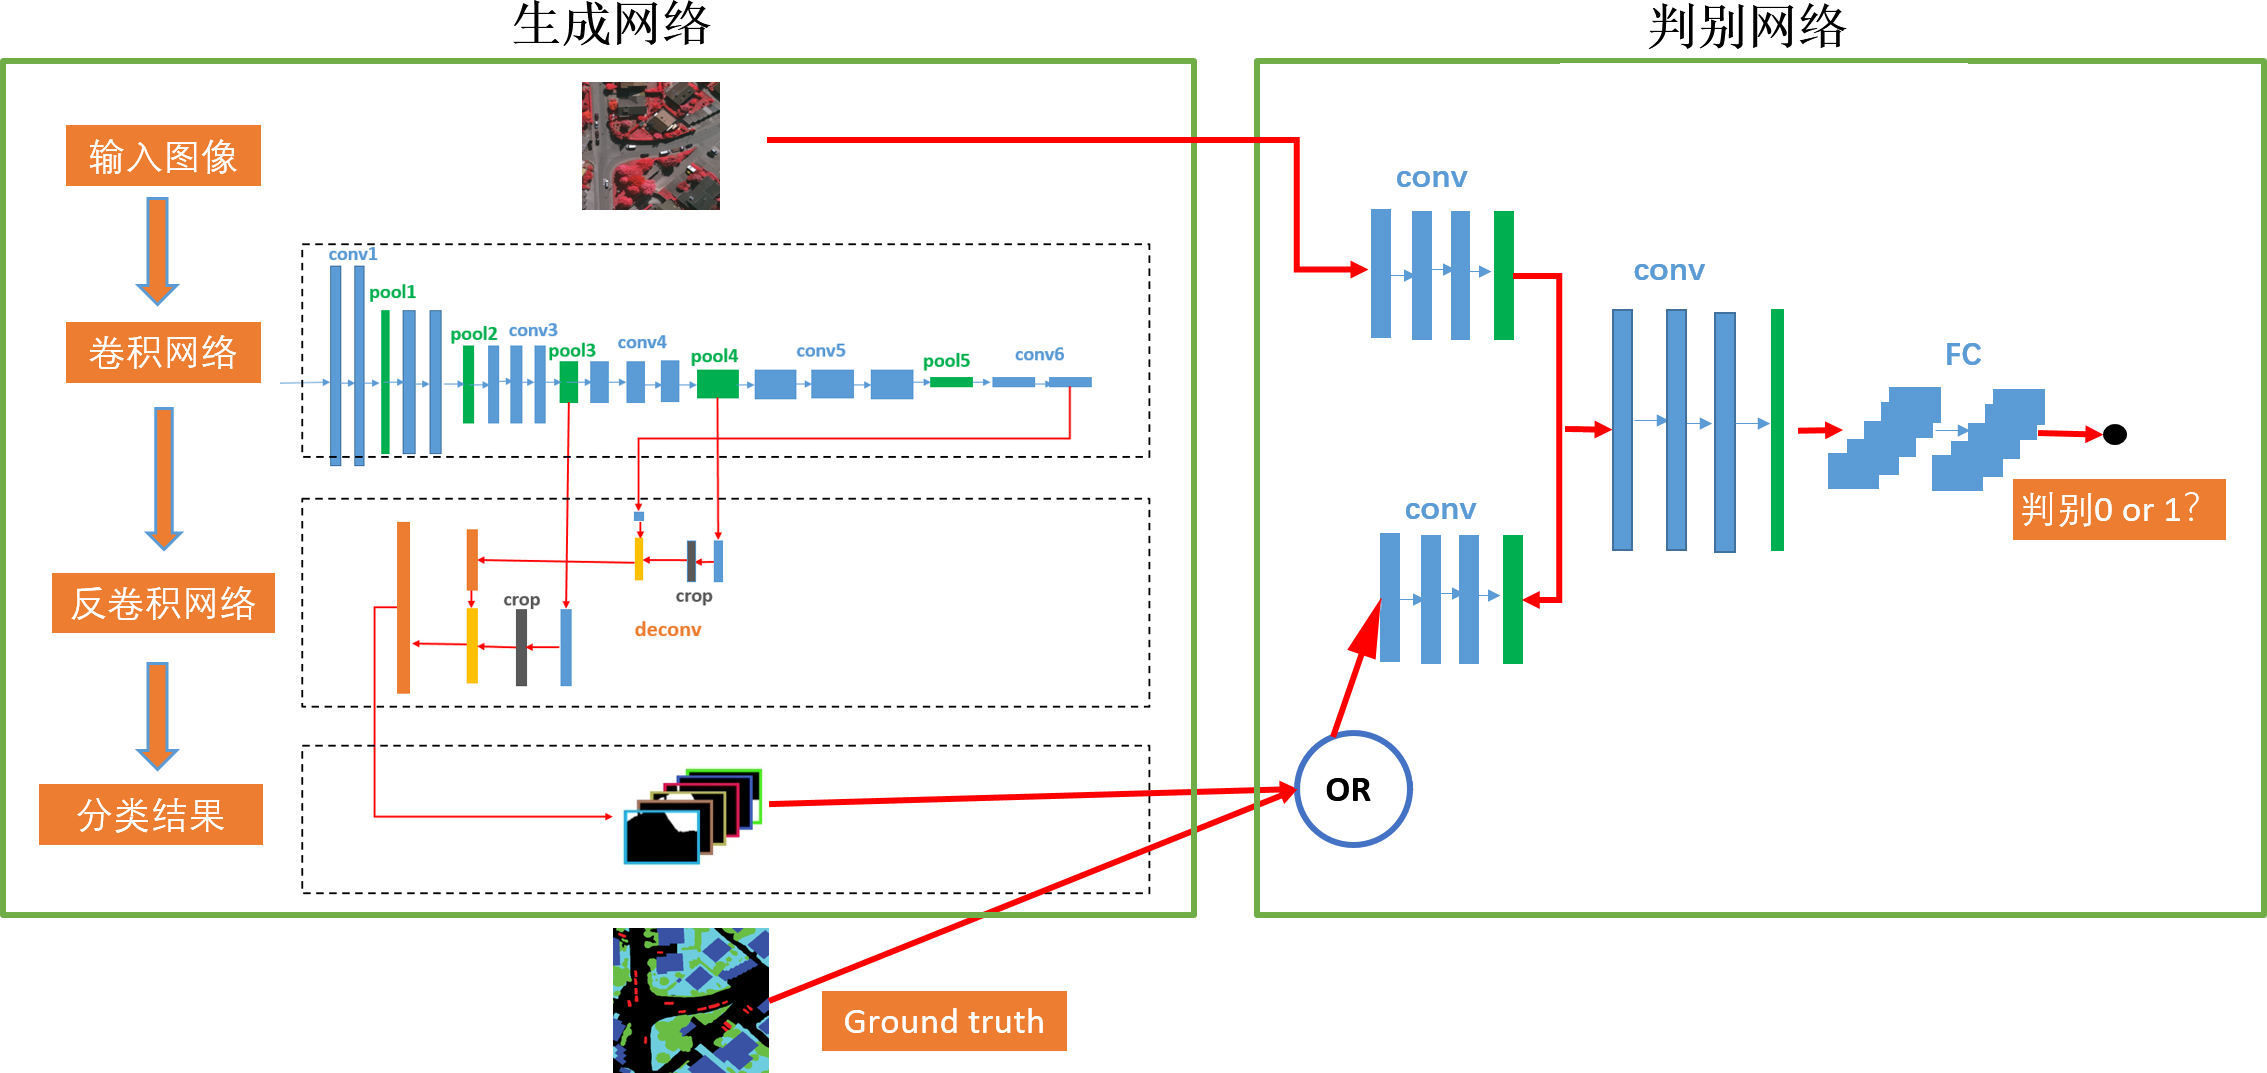
\includegraphics[width=1.05\textwidth]{figures/gan-fcn}}
    \caption{基于CGAN 的影像分类方法模型示意图}\label{fig:gan-fcn}
  \end{center}
\end{figure}

模型中使用二元分类损失(Binary classification loss, BCE)来度量判别网络。二元分类损失为二元交叉熵(cross entropy)函数,统计学中使用KL 散度衡量两个事件或分布中的不同,常用于计算代价损失,图像分类任务中最小化KL散度等价于最小化交叉熵,而交叉熵计算更简便\cite{de2005tutorial},因此文中用交叉熵来计算二元分类损失。交叉熵函数为分类预测概率值的负对数。二元交叉熵代价表达式如下:
\begin{equation}
  \label{eq:4-4}
  l_{bce} (\hat{z}, z) = -[z\log\hat{z} + (1-z)\log(1-\hat{z})]
\end{equation}

%+ (1-y_{ic})\log(1-\hat{y}_{ic})
生成网络是全卷积网络模型,其本质上是一个CNN 影像多分类模型。经典的多分类分割模型代价函数为多类别的交叉熵损失(multi-class entropy loss, MCE),分割模型输入为大小为$H\times W\times C$ 的图像,对图像做像素级预测分类,其多元交叉熵损失为:
\begin{equation}
  \label{eq:4-5}
  l_{mce} (\hat{y}, y) = -\sum_{i=1}^{H\times W}\sum_{c=1}^{C}y_{ic}\log\hat{y}_{ic}
\end{equation}
其中,$H$、$W$ 和$C$ 分别为图像的高度、宽度以及通道数。假定多分类问题中类标有$K$ 个取值,需要使用独热编码(One-hot encode)将图像类别标签编码为一个$K$ 维向量,借助Softmax 函数作为分类任务的输出层。Softmax 函数把神经网络分类输出转化为一组概率,且这组概率和为1。归属于类别$j$ 的概率为:
\begin{equation}
  \label{eq:4-6}
  p_j = \frac{e^{z_j}}{\sum_{k=1}^Ke^{z_k}}  \quad \forall j \in 1,2,\cdots, K
\end{equation}

假定有$N$ 张训练图片的数据集$X = \{x_1,x_2,\cdots, x_n \}$,对应的Ground truth 图标签集为$Y = \{y_1,y_2,\cdots, y_n \}$。输入图像大小为$H\times W\times C$(一般$C$ 取$3$),有$K$ 个类别的图像标签编码为$K$  维向量,即对第$i$ 张图像$x_i$,对应Ground truth 图有$y_j = [y_j^{(1)},y_j^{(2)}, \cdots, y_j^{(K)}]$。我们定义$g(x)$ 为输入图片$x$ 在生成网络分割模型下的预测输出,定义$d(x,y)\in [0,1]$ 为对抗网络判别图像标签$y$ 是输入图像$x$ 对应的Ground truth 图还是分割模型产生的分割结果的概率输出值。基于条件对抗网络框架的全卷积语义分割模型方法需要最小化分割模型的多分类交叉熵损失,同时最大化分割模型生成样本的判别概率。优化的目标代价函数为式\ref{eq:4-7}:
\begin{equation}
  \label{eq:4-7}
  L(\theta_g,\theta_d) = \sum_{n=1}^N \lbrace l_{mce} (g(x_n),y_n) - \lambda [l_{bce} (d(x_n,y_n),1) + l_{bce}(d(x_n,g(x_n)),0)] \rbrace
\end{equation}
式中$\theta_g$ 和$\theta_d$ 分别代表分割模型和判别模型网络参数,右式中第一项为分割模型的交叉熵损失,第二项为对抗网络中样本判别损失代价函数,$\lambda$ 为生成阶段与对抗阶段代价权衡常数且有$\lambda > 0$。模型训练时我们需要最小化式\ref{eq:4-7} 中的代价函数,从而迭代求解得到网络参数$\theta_g$ 和$\theta_d$。

% 通过前向传播,利用最终分割模型对待分类测试影像求解每个像素属于各个类别的概率值
当模型迭代收敛后,模型中的权值参数均得以确定,此时模型中生成网络部分已经具有优秀的图像分割识别能力。通过前向传播,利用最终分割模型对待分类测试影像求解每个像素属于各个类别的概率值,像素点所属类别概率值求采用式\ref{eq:4-6} 中Softmax 函数求解,接着根据argmax 函数计算像素点最大概率值对应类别维度,即为当前预测点的分类标签,影像$x$ 上任一像素点$i$ 所属类别标签$C_k$ 的计算方式如式\ref{eq:4-8}。
\begin{equation}
  \label{eq:4-8}
  C_k = \mathop{\arg\max}_{k \in K} p_k(x^{(i)}), \ k=1,2,\cdots,K
\end{equation}
类似地,对待分类影像所有像素点预测类别标签,即可实现该影像的分割。

\subsection{算法实现}
\label{subsec:firtst-2}

基于CGAN 的遥感影像分类方法需要交替训练生成网络和判别网络两部分,算法采取小批次的随机梯度下降方法优化CGAN 权值参数,Adam \cite{kingma2014adam} 优化器可以自适应调整学习率的大小,因此本算法使用Adam 优化器更新模型权重。基于CGAN 的影像分类模型更新迭代伪代码如算法~\ref{code:cgan} 所示。

\begin{algorithm}[!h]
  \caption{基于CGAN 的遥感影像分类方法伪代码}
  \begin{algorithmic}[1]
    \Require
    原始影像$X$; 影像标签$Y$;
    \Ensure
    生成样本;

    \textbf{模型训练:}
    \State VGGNet16 前五层权值初始化生成模型,判别器步数 $k= 1$,权衡因子$\lambda$, 初始学习率$\alpha$, Adam 动量 $\beta_1,\beta_2$。
    \For{模型迭代epoch 数}
    \State \textbf{判别器:}
    \For{$k$ 步 }
    \State 小批次抽样$m$ 张影像$\{x^1,x^2,\cdots, x^m\}$; 对应影像的真实标签$\{y^1,y^2,\cdots, y^m\}$;这$m$ 张影像在生成器中的输出$\{g(x^1),g(x^2),\cdots, g(x^m) \}$
    \State 使用Adam 优化器更新判别器的权重:
    $$
      \nabla_{\theta_d} \frac{1}{m} \sum_{i=1} ^m [\log(d(x^i,y^i)) + \log(1-d(x^i,g(x^i)) ]
    $$
    \EndFor
    \State \textbf{生成器:}
    \State 小批次抽样$m$ 张影像$\{x^1,x^2,\cdots, x^m\}$;
    \State 分割模型输出这$m$ 张影像分割结果$\{g(x^1),g(x^2),\cdots, g(x^m) \}$
    \State 使用Adam 优化器更新生成器的权重:
    $$
      \nabla_{\theta_g} \frac{1}{m} \sum_{i=1} ^m [\log(1-d(x^i,g(x^i))]
    $$
    \EndFor

    \textbf{模型预测:}
    \State 模型迭代收敛后,用生成器分割模型对测试影像预测分割结果,采用概率最大化预测类别标签:
    $$
      C_k = \mathop{\arg\max}_{k \in K} p_k(x^{(i)}), \ k=1,2,\cdots,K
    $$

  \end{algorithmic}
  \label{code:cgan}
\end{algorithm}


模型首先将影像数据划分为训练集和测试集,并赋值给对应变量。初始化CGAN 分割模型的超参数。在每次迭代内,分批次随机抽取生成分割图和Ground truth 图,分别与对应的原始影像对应拼接,联合输入判别模型,计算判别模型损失并更新判别模型相关权值参数。接着固定判别模型训练生成网络,计算模型损失并更新生成器参数权重,完成网络的一次迭代。模型收敛后即用生成分割模型对测试集影像进行处理,得到模型分割结果图。


\section{实验数据介绍与预处理}
\label{sec:second}

\subsection{Vaihingen 数据介绍}
\label{sec:second-1}
本章实验数据源为ISPRS(国际摄影测量及遥感探测学会)提供的Vaihingen 高分辨率遥感影像数据\footnote{Vaihingen 数据集官网链接:http://www2.isprs.org/commissions/comm3/wg4/detection-and-reconstruction.html}。Vaihingen 数据集由德国测量和遥感协会(DGRF)于2010年使用空中数字摄像机拍摄,拍摄区域为半农村地区的德国斯图加特市法伊欣根市镇(Vaihingen),影像空间分辨率为$0.09m$。如图\ref{fig:vaihingen}(a) 所示为Vaihingen 数据整体图,整个数据被划分为33幅大小不一的图像,其中带有真实地面数据的影像为16幅。Vaihingen 数据包含三个波段(近红外-红-绿)的正射影像数据(Orthophoto)、数字地表模型(Digital Surface Model,DSM)数据以及拍摄区域真实地物分类结果(Ground truth)。图\ref{fig:vaihingen}(b-d) 分别为该影像某一区域的正射影像、DSM高程、Ground truth 图。

\begin{figure}[!htb]
  \centering
  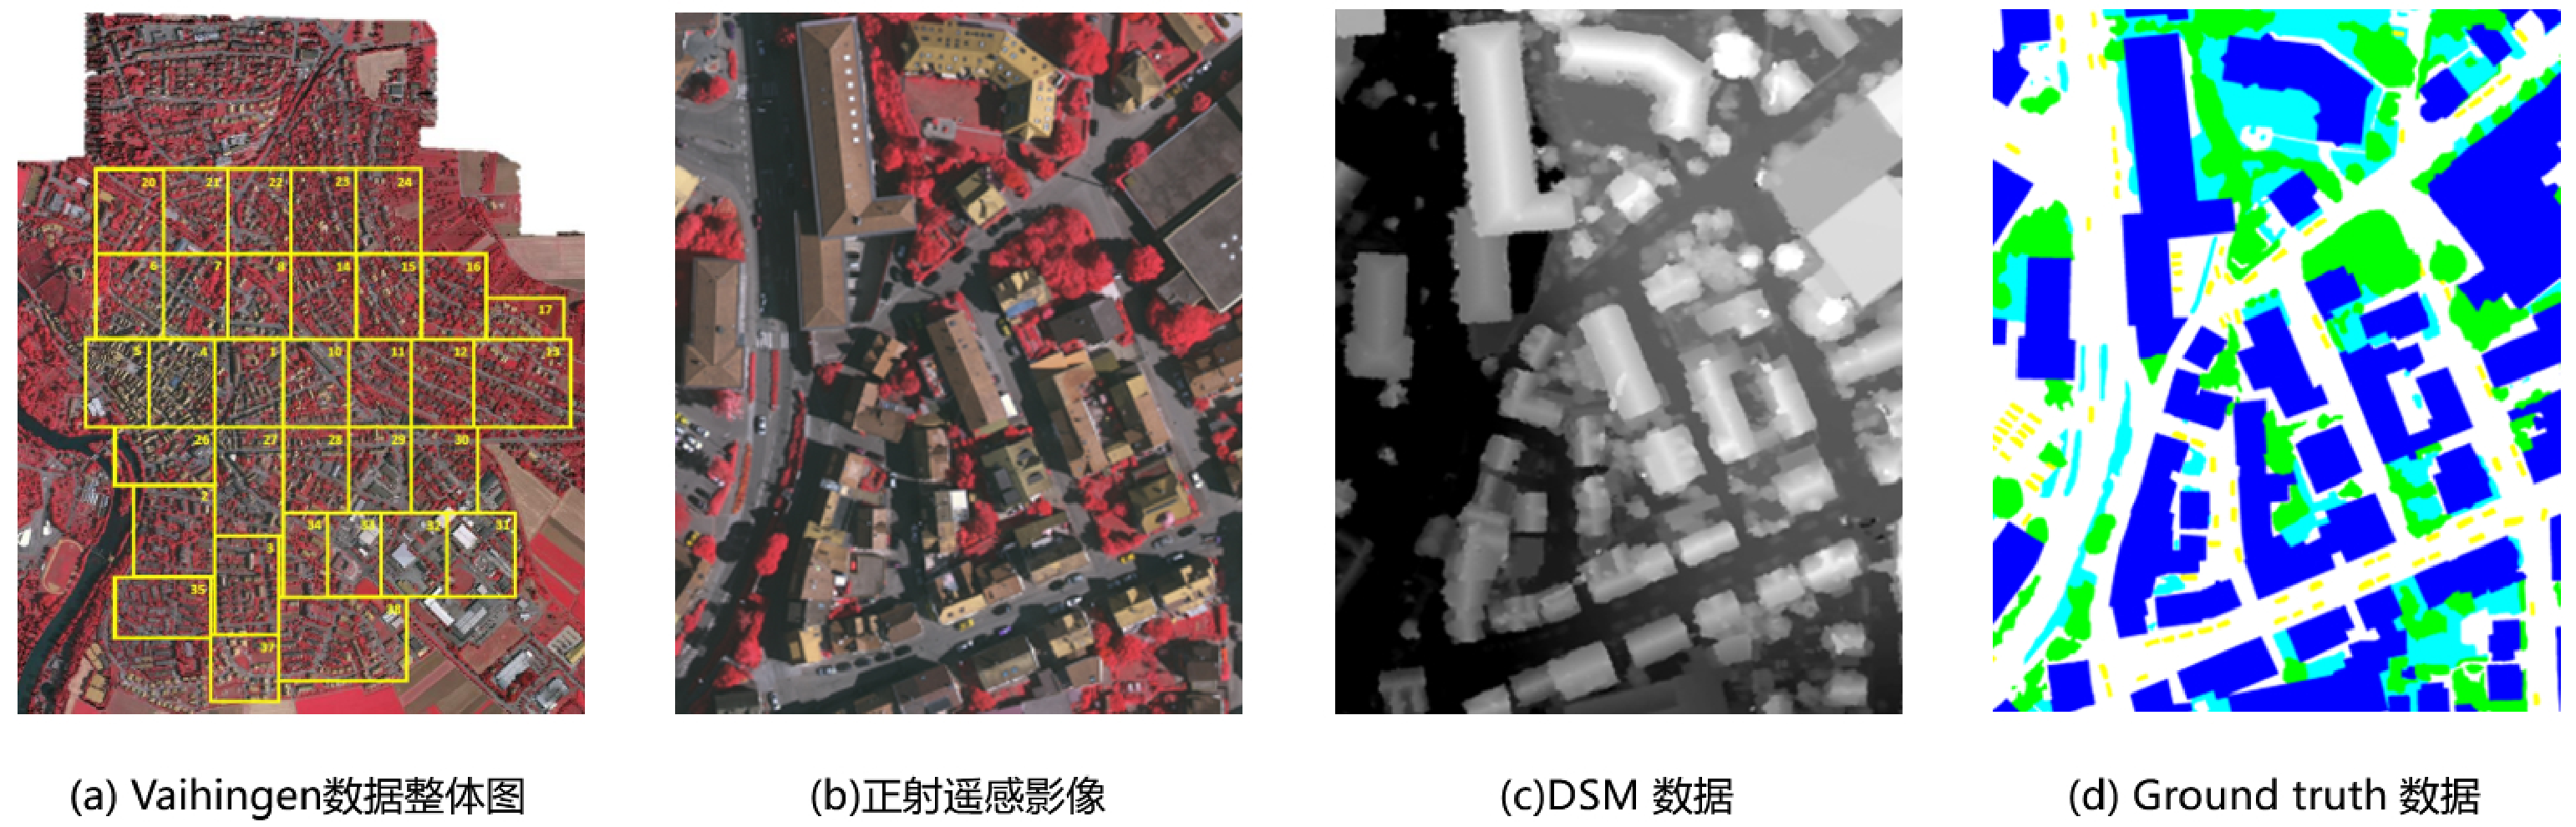
\includegraphics[width=0.98\textwidth]{figures/vaihingen2}
  \caption{Vaihingen 影像数据}\label{fig:vaihingen}
\end{figure}

Vaihingen 地区影像依据领域专家人工解译结果划分为地面、低矮植被、树木、建筑物、车辆、背景六类地物。Ground truth 图中六类地物的类别和对应颜色分别如表\ref{tab:vaih_gt} 所示。

\begin{table}[!htbp]
  \caption{Vaihingen 数据类别标签颜色对照表}\label{tab:vaih_gt}
  \centering
  \footnotesize

  \begin{tabular}{p{2cm}p{2cm}p{3cm}p{2cm}}
    \toprule
    地物类别 & 颜色 & 色彩值(R,G,B)   & 类别标签 \\
    \midrule
    地面     & 白色 & $(255,255,255)$ & 0        \\
    低矮植被 & 青色 & $(0,255,255)$   & 1        \\
    树木     & 绿色 & $(0,255,0)$     & 2        \\
    建筑物   & 蓝色 & $(0,0,255) $    & 3        \\
    车辆     & 黄色 & $(255,255,0)$   & 4        \\
    背景     & 红色 & $(255,0,0) $    & 5        \\
    \bottomrule
  \end{tabular}
\end{table}

\subsection{数据预处理}
\label{sec:second-2}

\subsubsection*{1. 波段组合}
Vaihingen 高分辨率影像空间、几何信息丰富,但正射影像光谱波段只有三个,仅使用正射影像数据无法完备有效地提取影像特征。而对于光谱相似区域的地物,如地面、建筑物、阴影等,更加难以区分,DSM 数据包含了地形、桥梁、房屋住宅和树木等高度地面高程信息,对模型区分地表建筑物、地面影像、不同高度植被一定程度上能提供帮助。Vaihingen 影像的DSM 包含一个波段,其像素值表示高度值。因此,将Vaihingen 数据的DSM 作为额外的波段附加在正射影像波段后,参与模型训练。

\subsubsection*{2. 数据集划分}
Vaihingen 数据中带有Ground truth 图的影像共有16张,实验中随机选取12张影像(标号为$1,5,7,11,15,17,21,26,28,30,32$ 和$37$)作为模型训练集,另外4张影像(标号为$3,13,23,34$)作为模型测试集。将影像Ground truth 图由RGB 图像转化为1维类别标签标签,各地物类别与对应的标签如表\ref{fig:vaihingen} 所示。

\subsubsection*{3. 数据归一化}
Vaihingen 影像数据集各通道的像素点取值在$[0,255]$ 范围内,像素点的分布范围较广,如果直接输入神经网络容易引起神经元输出因输入绝对值过大而饱和的现象,从而整个网络难以收敛。所以需要对图像数据做归一化处理,即将图像像素点取值从$[0,255]$ 范围映射到一个较小的变化范围,把有量纲表达式变为无量纲表达式,加快训练网络的收敛速度。

图像常用归一化方法有均值方差标准化和最大最小值归一化这两种。均值方差标准化又叫做z-score 标准化,其处理过程是原始数据与平均值的差再除以标准差。如式\ref{eq:4-9} 所示,
\begin{equation}
  \label{eq:4-9}
  z = \frac{x-\mu}{\sigma}
\end{equation}
式中$x$ 为原始输入数据,$\mu$ 和$\sigma$ 分别为数据的平均值和标准差,$z$ 为$x$ z-score 标准化后的输出。 经过z-score 标准化后数据服从均值为0、方差为1的正态分布,该方法多用于预处理没有明显边界的数据。

最大最小值归一化方法则是通过线性函数转换,将某变化范围内数据映射到$[0,1]$ 之间,线性映射过程如式\ref{eq:4-10} 所示:
\begin{equation}
  \label{eq:4-10}
  y = \frac{x-x_{min}}{x_{max}-x_{min}}
\end{equation}
式中$x$ 为原始输入数据,$x_{max}$ 和$x_{min}$ 分别为数据的最大值和最小值,$y$ 为$x$ 最大最小值归一化后的输出。

本实验中采用最大最小值归一化方法对高分影像做归一化处理,将影像像素值从$[0,255]$ 映射到$[0,1]$ 之间,加快神经网络的训练和收敛速度。

\subsubsection*{4. 样本选取与数据增强}
高分影像单张图像尺寸通常很大,直接送入神经网络计算量太大,无法完成训练。Vaihingen 单张影像尺寸大约为 $2563 \times 2049$,不能直接用于网络训练。本实验中对原始影像进行裁切处理,将影像裁剪为大小$256 \times 256$ 的图像块作为模型训练集样本。可有效降低网络训练计算量,避免内存溢出。

\begin{figure}[!htbp]
  \centering
  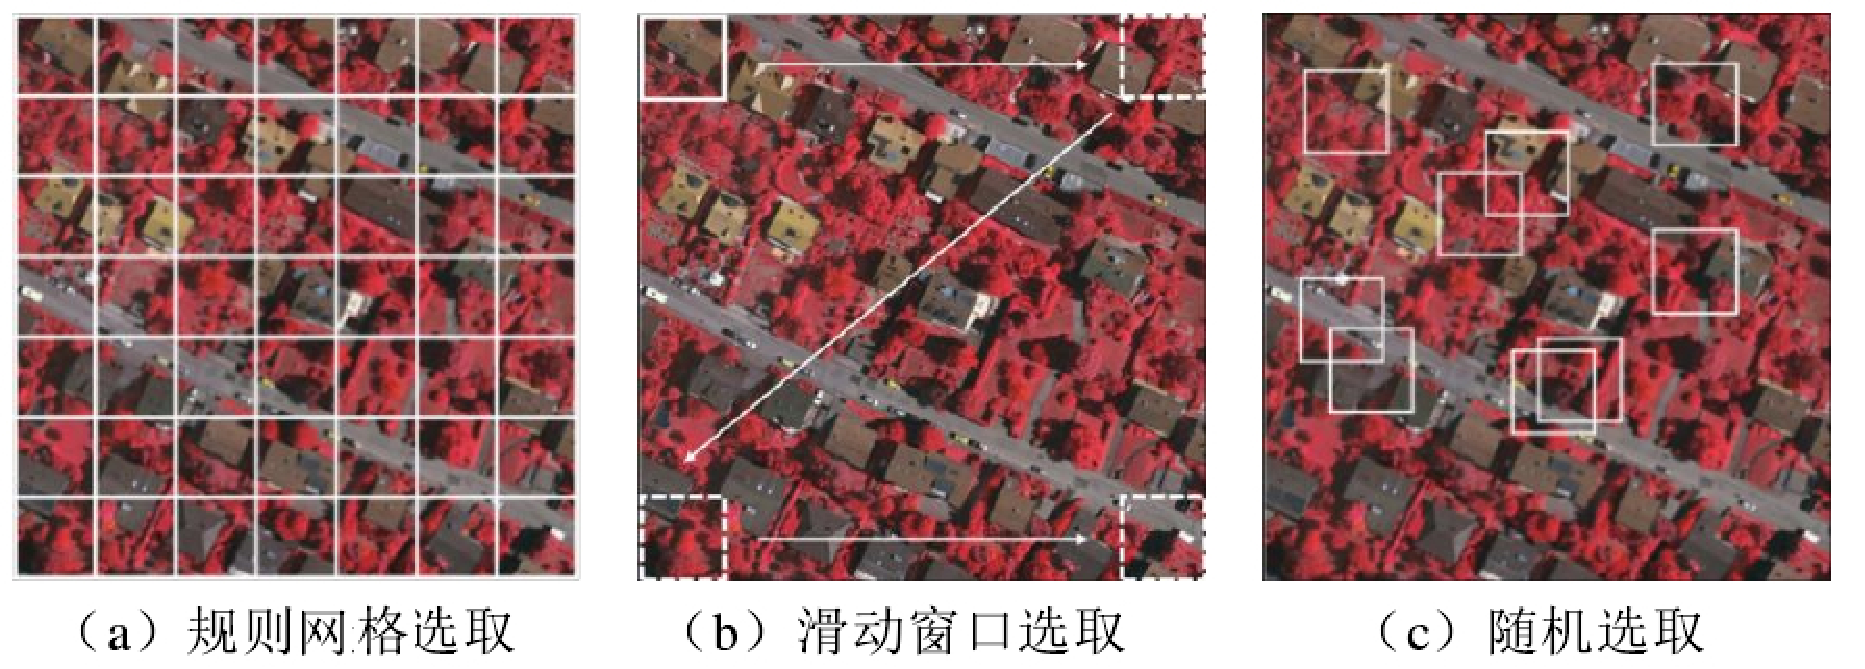
\includegraphics[width=0.8\textwidth]{figures/sample_data}
  \caption{图像裁剪方式}\label{fig:sample_data}
\end{figure}

常用图像裁剪方式有规则网格选取、滑动窗口裁剪和随机选取。规则网格选取是使用大小为$256 \times 256$ 的网格切分影像,这种划分方式得到的样本量有限。滑动窗口裁剪方法以特定的移动间隔在原始影像上剪裁得到训练样本。文中采用滑动窗口尺寸为$256 \times 256$,滑动窗口样本受滑动间隔尺度影像,滑动间隔小得到的冗余影像过多,滑动间隔大则会丢失影像许多特征信息。随机选取则是使用$256 \times 256$ 的裁剪窗口在原始影像上裁切获得样本。这种方法灵活便捷,能够有效利用遥感影像的信息,且裁剪出大量的训练样本。三种裁剪方式如图\ref{fig:sample_data} 所示。

本文实验中训练样本采用随机裁剪选取方式获得,测试样本采用规则网格选取方式获得。获取裁剪样本时也对同一区域的DSM、Ground truth 图数据进行裁切,保证输入数据与类别标签的一致性。

另外,为了获取更多的有效数据,增强网络模型的泛化能力,这里对训练样本做数据增强(Data augmentation)处理。数据增强是通过一些几何变换(如平移、旋转和翻转)从已有训练样本图像生成一些新的样本,来扩大训练数据集。文中对上一步裁剪获得的训练样本做镜像对称,水平翻转处理,来扩大已有训练样本集,增强模型泛化能力。

本小节对Vaihingen 有标签的16块影像数据处理,其中12张影像得到训练集样本图像$5760$ 幅,用于测试集的4 张影像经规则网格选取法得到大小为$256 \times 256$ 的测试图像合计$320$ 张。




\section{实验结果与分析}
\label{sec:third}
\subsection{实验环境}
\label{sec:third-1}
本章实验电脑为思腾合力IR4200 服务器,其主要参数如下:CPU 为两块 Intel Xeon E5-2690 2.9GHz 8核 16线程正式版处理器,内存为128G 容量8通道DDR4 服务器内存,GPU 为技嘉 1080Ti,显存 12G。实验中使用 Ubuntu 16.04 LTS 操作系统,编程语言为Python 3.5,神经网络模型采用谷歌开源框架Tensorflow 编程实现,Tensoflow 版本为1.5.0。

\subsection{评价指标}
\label{sec:third-2}
本节实验分别通过定性和定量两种指标来评估影像分割结果。定性即人工主观对测试图像的分割结果图做出评判,定量分析则使用图像分割中常用到的两种指标:

(1)总体精度(Overall accuracy,OA),即遥感影像分类精度最直观的评价指标,其值为影像中被正确分类的像元个数除以总像元个数,其计算方式如下式:
\begin{equation}
  \label{eq:4-11}
  OA = \frac{1}{A_{\mbox{总}}}  \sum_{k=1}^K a_{kk}
\end{equation}
式中$A_{\mbox{总}}$ 为真实地物像元总数,$K$ 为地物类别数,$a_{kk}$ 第$k$ 类地物被正确分类的像元数。

(2)平均交并比(Mean Intersection over union, mIoU),IoU 是影像中真实标签与预测分割结果两者交集与并集的比值,mIoU 是图像语义分割领域最常用的准确度度量方法,它分别对影像每个地物类别计算IoU,然后再对所有地物类别的IoU 求均值。IoU 的计算方式如式\ref{eq:4-12}:
\begin{equation}
  \label{eq:4-12}
  IoU = \frac{\mbox{预测结果} \cap \mbox{真实标签}}{\mbox{预测结果} \cup \mbox{真实标签}}
\end{equation}
影像所有类别地物的mIoU 的计算方式如式\ref{eq:4-13}:
\begin{equation}
  \label{eq:4-13}
  mIoU = \frac{1}{K}  \sum_{i=1}^K \frac{a_{ii}}{\sum_{j=1}^Ka_{ij} + \sum_{j=1}^Ka_{ji} -a_{ii}}
\end{equation}
式中$a_{ij}$ 表示第$i$ 类地物被错分为第$j$ 类的像元个数,$a_{ji} $ 表示第$j$ 类地物被错分为第$i$ 类的像元个数,$a_{ii}$ 表示第$i$ 类地物正确预测的像元个数。


\subsection{网络参数}
\label{sec:third-3}

本节实验中输入图像为 $256\times 256\times 4$ 的4波段融合影像(近红外、红、绿、DSM),生成网络中的分割模型权值使用ImageNet 上预训练好的基于VGGNet16\cite{simonyan2014very} 的全卷积网络权值初始化,式\ref{eq:4-7} 中GAN 模型中的目标函数权衡因子为$\lambda = 2$ ,使用Adam \cite{kingma2014adam} 优化器计算梯度更新,Adam 优化器具有自适应的学习率,初始学习率为 $\alpha = 10^{-4}$,梯度动量一阶和二阶矩估计指数衰减率分别初始化为$\beta_1 = 0.9$ 和$\beta_2 = 0.9999$,$\epsilon = 10^{-8}$ 防止除数为$0$。实验中设置批大小(Batch size) 为$128$, epoch 为$150$ 时能取得更好的训练效果。

模型生成器G 中的网络压缩部分由五个卷积模块堆叠而成,其作用是逐层提取影像特征。每个卷积模块均包含$2/3$ 个卷积层和$1$ 个尺寸$2\times 2$最大池化层,为了保证卷积前后特征图尺寸不变,所有卷积层均采用边界填充,最大池化层使得特征图尺寸缩小为池化前的一半。生成器G 中反卷积恢复为四个反卷积的上采样模块,其作用是逐层扩大特征图大小、恢复影像细节信息。每个上采样模块中包含一次反卷积操作,反卷积生成两倍维度的特征图,再接两层卷积层提取特征。最后通过一个$1\times 1$ 大小的$1$ 维卷积层将特征图维度降维$1$,通过Softmax 函数输出预测结果的像素类别。另外,在反卷积中使用跳层连接网络压缩部分与反卷积层特征图大小相同的卷积层,从而将影像低阶特征和高阶特征融合,保证更精细的分割结果。

\begin{longtable}[!htbp]{c|c|cccccc}
  \caption{基于CGAN 框架的全卷积分割模型参数表}\label{tab:model_param}                                                                                                 \\
  \toprule
  网络模型                 & 结构                       & Levels                   & 网络层     & 该层输出尺寸                & 卷积核               & 步长 & 激活函数 \\
  \midrule
  \endfirsthead
  % \multicolumn{8}{r}{续\autoref{tab:model_param}}\\
  \multicolumn{8}{c}{(接上页)}                                                                                                                                         \\
  \toprule
  网络模型                 & 结构                       & Levels                   & 网络层     & 该层输出尺寸                & 卷积核               & 步长 & 激活函数 \\
  \midrule
  \endhead
  \bottomrule
  \multicolumn{8}{c}{(接下页)}
  \endfoot
  \bottomrule
  \endlastfoot
  \multirow{30}*{生成器G}  & G-输入                     & {level 0 }               &            & $256\times 256\times 4   $  &                      &      &          \\
  \cline{2-8}
                           & \multirow{17}*{卷积压缩}   & \multirow{2}*{level 1}   & conv1\_1   & $256\times 256\times 64$    & $3\times 3/64$       & 1    & ReLU     \\
                           &                            &                          & conv1\_2   & $256\times 256\times 64$    & $3\times 3/64$       & 1    & ReLU     \\
  \cline{3-8}
                           &                            & \multirow{3}*{{level 2}} & pool2\_1   & $128\times 128\times 64  $  & $   2\times 2/-    $ & 2    & --       \\
                           &                            &                          & conv2\_1   & $128\times 128\times 128 $  & $     3\times 3/128$ & 1    & ReLU     \\
                           &                            &                          & conv2\_1   & $128\times 128\times 128 $  & $     3\times 3/128$ & 1    & ReLU     \\
  \cline{3-8}
                           &                            & \multirow{4}*{level 3}   & pool3\_1   & $64\times 64\times 128   $  & $ 2\times 2/-      $ & 2    & --       \\
                           &                            &                          & conv3\_1   & $64\times 64\times 256   $  & $ 3\times 3/256    $ & 1    & ReLU     \\
                           &                            &                          & conv3\_2   & $64\times 64\times 256   $  & $ 3\times 3/256    $ & 1    & ReLU     \\
                           &                            &                          & conv3\_3   & $64\times 64\times 256   $  & $ 3\times 3/256    $ & 1    & ReLU     \\
  \cline{3-8}
                           &                            & \multirow{4}*{level 4}   & pool4\_1   & $32\times 32\times 256   $  & $ 2\times 2/-      $ & 2    & --       \\
                           &                            &                          & conv4\_1   & $32\times 32\times 512   $  & $ 3\times 3/512    $ & 1    & ReLU     \\
                           &                            &                          & conv4\_2   & $32\times 32\times 512   $  & $ 3\times 3/512    $ & 1    & ReLU     \\
                           &                            &                          & conv4\_3   & $32\times 32\times 512   $  & $ 3\times 3/512    $ & 1    & ReLU     \\
  \cline{3-8}
                           &                            & \multirow{4}*{level 5}   & pool5\_1   & $16\times 16\times 512   $  & $ 2\times 2/-      $ & 2    & --       \\
                           &                            &                          & conv5\_1   & $16\times 16\times 512   $  & $ 3\times 3/512    $ & 1    & ReLU     \\
                           &                            &                          & conv5\_2   & $16\times 16\times 512   $  & $ 3\times 3/512    $ & 1    & ReLU     \\
                           &                            &                          & conv5\_3   & $16\times 16\times 512   $  & $ 3\times 3/512    $ & 1    & ReLU     \\
  \cline{2-8}
                           & \multirow{12}*{反卷积恢复} & \multirow{3}*{level 6}   & deconv6\_1 & $32\times 32\times 512   $  & $ 4\times 4/512    $ & 2    & ReLU     \\
                           &                            &                          & conv6\_1   & $32\times 32\times 512   $  & $ 3\times 3/512    $ & 1    & ReLU     \\
                           &                            &                          & conv6\_2   & $32\times 32\times 512   $  & $ 3\times 3/512    $ & 1    & ReLU     \\
  \cline{3-8}
                           &                            & \multirow{3}*{level 7}   & deconv7\_1 & $64\times 64\times 256   $  & $ 4\times 4/256    $ & 2    & ReLU     \\
                           &                            &                          & conv7\_1   & $64\times 64\times 256   $  & $ 3\times 3/256    $ & 1    & ReLU     \\
                           &                            &                          & conv7\_2   & $64\times 64\times 256   $  & $ 3\times 3/256    $ & 1    & ReLU     \\
  \cline{3-8}
                           &                            & \multirow{3}*{level 8}   & deconv8\_1 & $128\times 128\times 128 $  & $ 4\times 4/128    $ & 2    & ReLU     \\
                           &                            &                          & conv8\_1   & $128\times 128\times 128 $  & $     3\times 3/128$ & 1    & ReLU     \\
                           &                            &                          & conv8\_2   & $128\times 128\times 128 $  & $     3\times 3/128$ & 1    & ReLU     \\
  \cline{3-8}
                           &                            & \multirow{3}*{level 9}   & deconv9\_1 & $256\times 256\times 64  $  & $ 4\times 4/64     $ & 2    & ReLU     \\
                           &                            &                          & conv9\_1   & $256\times 256\times 64  $  & $     3\times 3/64 $ & 1    & ReLU     \\
                           &                            &                          & conv9\_2   & $256\times 256\times 64  $  & $    3\times 3/64  $ & 1    & ReLU     \\
  \cline{2-8}
                           & G-输出                     &                          & conv10\_1  & $256\times 256 \times 1   $ & $    1\times 1/1  $  & 1    & Softmax  \\
  \cline{1-8}
  \multirow{10}*{判别器D } & D-输入                     &                          &            & $256\times 256\times 5   $  &                      &      &          \\
  \cline{2-8}
                           & \multirow{8}*{分类网络}    & \multirow{2}*{level 11}  & conv11\_1  & $256\times 256\times 32$    & $3\times 3/32$       & 1    & ReLU     \\
                           &                            &                          & conv11\_2  & $256\times 256\times 32$    & $3\times 3/32$       & 1    & ReLU     \\
  \cline{3-8}
                           &                            & \multirow{3}*{level 12}  & pool12\_1  & $128\times 128\times 32$    & $2\times 2/-$        & 1    & --       \\
                           &                            &                          & conv12\_1  & $128\times 128\times 32$    & $3\times 3/32$       & 1    & ReLU     \\
                           &                            &                          & conv12\_2  & $128\times 128\times 32$    & $3\times 3/32$       & 1    & ReLU     \\
  \cline{3-8}
                           &                            & \multirow{3}*{level 13}  & pool3\_1   & $64\times 64\times 32   $   & $ 2\times 2/-      $ & 2    & --       \\
                           &                            &                          & FC13\_1    & $64\times 64\times 32   $   & $ 3\times 3/32    $  & 1    & --       \\
                           &                            &                          & FC13\_2    & $64\times 64\times 32   $   & $ 3\times 3/32    $  & 1    & --       \\
  \cline{2-8}
                           & G-输出                     &                          &            & $1\times 1   $              &                      &      & Sigmoid  \\
\end{longtable}

模型判别器D 中是一个经典的二分类神经网络,网络输入为$5$ 维数据(4波段影像 + 1维真实类别图或4波段影像 + 生成器G 生成分割结果图),模型由两个卷积结构后接两个全连接层组成,通过Sigmoid 函数判别当前输出结果为1 或0 。

基于CGAN 框架的全卷积分割模型详细的网络结构与参数权值如表\ref{tab:model_param} 所示,交替训练生成器G 和判别器D 完成网络各权值参数的学习。


\subsection{结果与分析}
\label{sec:third-3}

本章提出的基于CGAN 的影像分类方法将条件生成对抗的思想引入全卷积分类方法中,利用CGAN 对生成样本与真实标签的差异纠正能力,能够获得更准确的地物分类边界,且保持同类地物类内像素点类别一致性。实验中采用的是融合正射三波段影像和DSM 数据的四波段数据,实验对比的基准方法为经典的FCN 语义分类方法。下面分别从精确量化和目视评估两个角度对Vaihingen 数据集上的地物分割识别结果进行比较。

表\ref{tab:seg_refult} 比较了新提出的基于CGAN 的影像分类模型和FCN 模型的分类精度,分别统计了地面、低矮植被、树木、建筑物、车辆五类地物(背景未计算)的分类精度,整幅图片中五类地物总体精度和mIoU 指标。从分类精度可知,两种方法对地面、树木和建筑物均有较好的识别精度,低矮植被易与背景中阴影混淆,故整体识别精度较低,车辆分类精度也不高,这与样本中车辆所占像素面积少,存在该类别样本数不多相关。文中提出的基于CGAN 的分类方法在“建筑物”这个类别地物识别精度最高,为 $87.64\%$ ,相比FCN 分类方法的$83.96\%$ ,有约$4\%$ 的绝对精度提升。而对FCN 分类中精度较低的“低矮植被”地物,分类精度由$63.39\%$ 大幅提升到$74.47\%$,该类别识别精度提升幅度达$10\%$,提升原因一方面是方法中使用DSM 波段数据能量化区分低矮植被与阴影的高度特征差异,较好得区分二者,另一方面则是基于CGAN 的分类方法对地物的边界有更准确的生成能力。本文提出基于CGAN 的分类方法OA 为$80.15\%$,mIoU 为$61.83\%$,相比FCN 分类算法中$78.48\%$ 的OA 和$58.42\%$ 的mIoU, 均有一定程度的提升。

\begin{table}[htbp]
  \caption{Vaihingen 数据分类精度评估表}\label{tab:seg_refult}
  \centering
  \begin{tabular}{ccccccccc}
    \toprule
    方法              & 地面      & 低矮植被  & 树木      & 建筑物    & 车辆      & OA        & mIoU               \\
    \midrule
    FCN 分类方法      & $81.14\%$ & $63.39\%$ & $79.52\%$ & $83.96\%$ & $62.39\%$ & $78.48\%$ & $58.42\%$          \\
    基于CGAN 分类方法 & $83.78\%$ & $74.47\%$ & $82.40\%$ & $87.64\%$ & $78.83\%$ & $80.15\%$ & \textbf{$61.83\%$} \\
    \bottomrule
  \end{tabular}
\end{table}

\begin{figure}[htb]
  \centering
  \includegraphics[width=0.9\textwidth]{figures/seg_result}
  \caption{影像分类的可视化结果}\label{fig:seg_result}
\end{figure}


图\ref{fig:seg_result} 为本文提出的基于CGAN 的分类方法和FCN 分类方法分别在三组测试影像上分类预测的可视化结果。图\ref{fig:seg_result}(a) 为一居民住宅区,参照真实地物类别的Ground truth 图,相比FCN 分类方法,基于CGAN 的影像分类方法在处理图中建筑物与房屋阴影的分割边界时,能更好地将阴影划分到背景中,更加准确地将住宅等建筑物识别为一个整体,从易混淆的阴影中区分开。图\ref{fig:seg_result}(b) 则是一处停车场周边影像图,对形态不一、位置各异的车辆进行识别预测是关键。如左下角部分停靠在树木下的两排车辆,一些车辆与地面特征相似,区分度较小,FCN 分类算法无法识别出这些“车辆”,直接将车错分为背景,而基于CGAN 的分类方法则对停靠的车辆尽可能准确的进行了识别预测。相比前者,尽可能地找出了停靠在树木阴影下的车辆。图\ref{fig:seg_result}(c) 为一处树木与建筑物环绕区域,对“建筑物”、“低矮植被”以及“树木”三类地物的边界明确划分成为预测分类的难点。如图正上方区域房屋环绕的树木与低矮植被区域,基于CGAN 的分类方法将图中的“树木”与“低矮植被”进行了区分,而FCN 的分类方法则将“低矮植被”识别为“树木”。综合上面三组图像的分类结果,文中提出的基于CGAN 的影像分类方法相比FCN 分类方法能够区分特征相近地物类别,生成更准确的分割边界。


\begin{figure}[!htb]
  \centering
  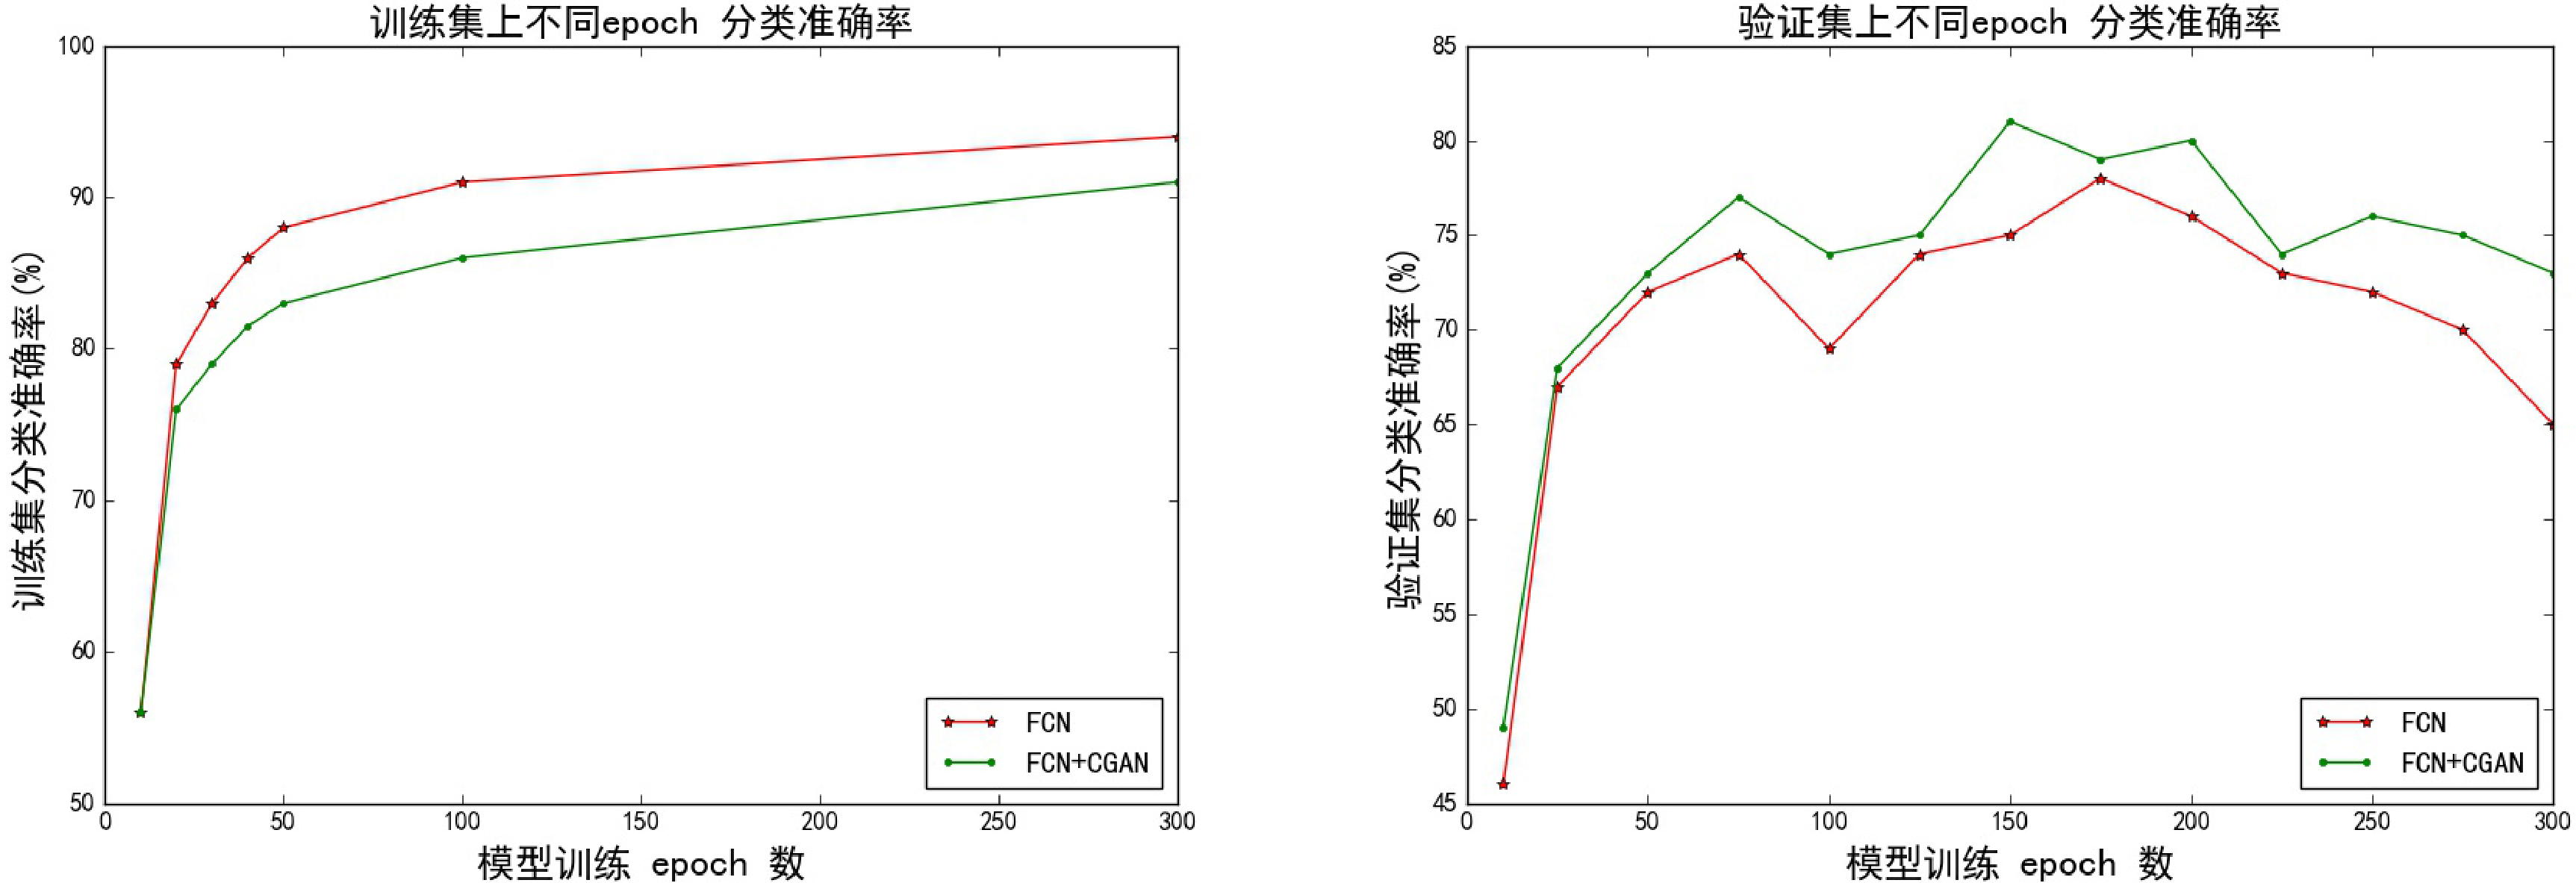
\includegraphics[width=\textwidth]{figures/epoch_acc}
  \caption{两种模型训练集和验证集准确率随模型迭代次数变化示意图}\label{fig:epoch_acc}
\end{figure}

图\ref{fig:epoch_acc} 所示为基于CGAN 影像分类方法和标准FCN分类方法模型迭代过程中训练集和测试集准确率随迭代epoch数变化示意图。从折线图的结果可知,基于CGAN 影像分类方法相比基准FCN 分类方法有更好的泛化能力,即随着epoch 次数变得很大($200\sim 300$),FCN 验证测试集上的分类精度下降明显,而基于CGAN 分类方法下降趋势较平缓。此外,可知当epoch 次数为150次附近时,模型在验证测试集上能获得最优的分类效果。

\begin{figure}[!htb]
  \centering
  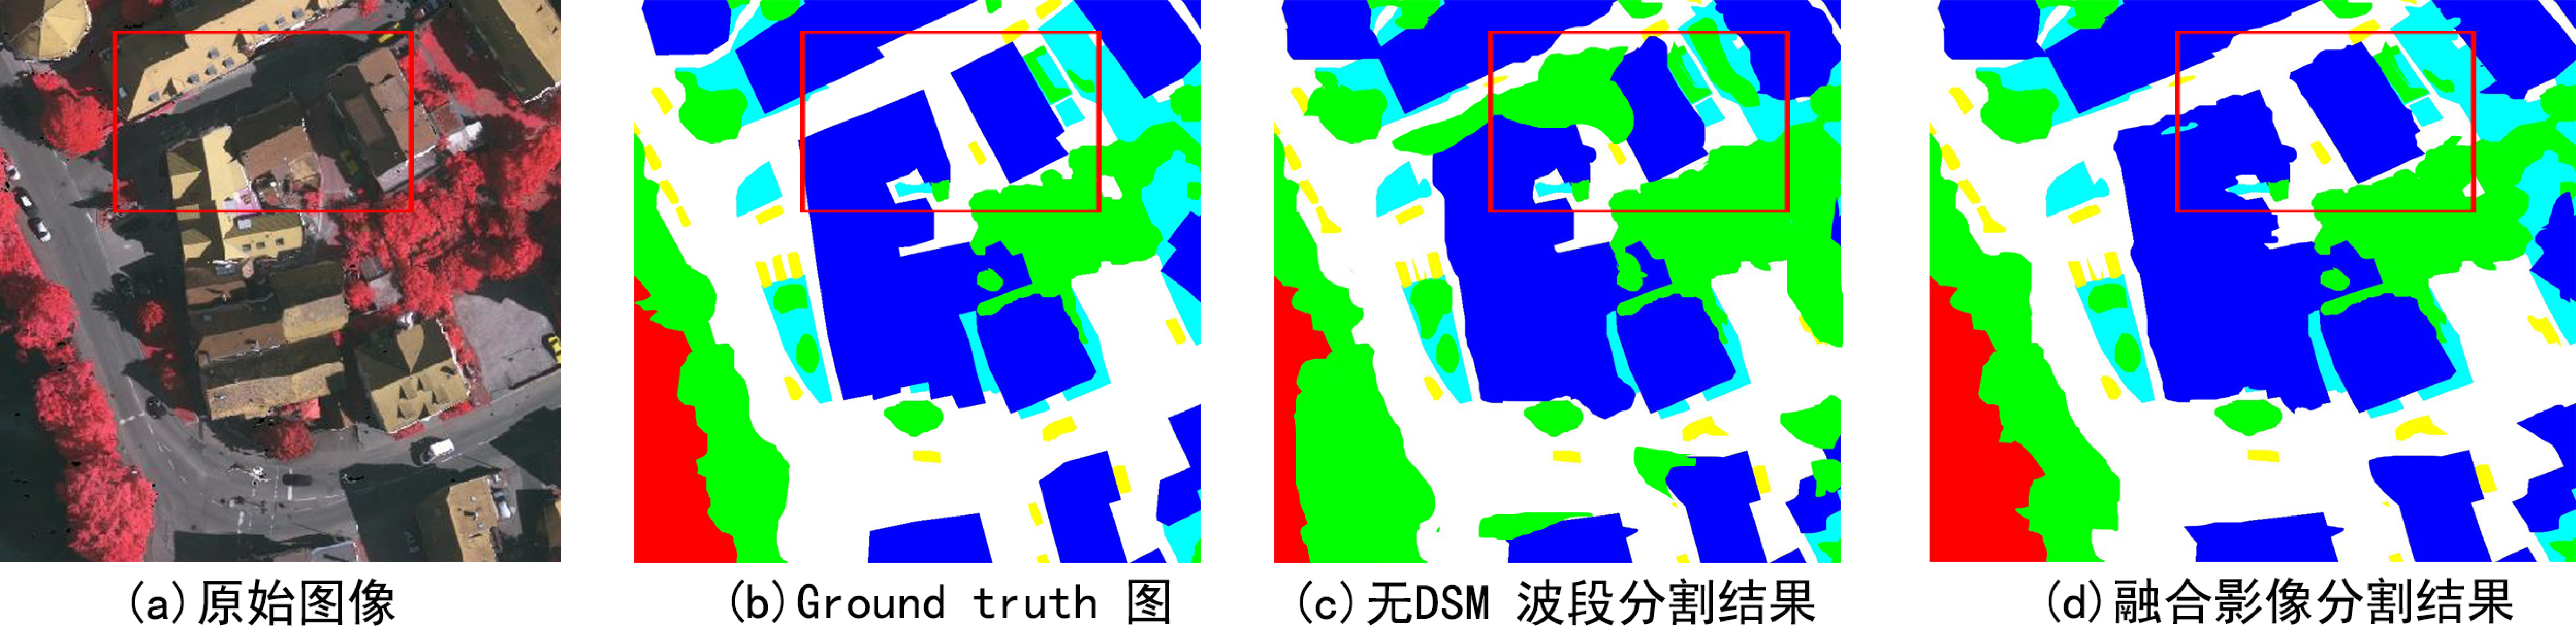
\includegraphics[width=0.9\textwidth]{figures/dsm_affect}
  \caption{DSM 波段对影像分类结果的影响}\label{fig:dsm_affect}
\end{figure}

文中使用的训练样本为三波段正射影像与一波段DSM 的融合数据。下文实验比较了DSM 数据对实验结果的影响。DSM 数据包含地形和地物高度等相关高程信息,“道路”、“低矮植被”和“建筑物”容易受不同地形、高度变化导致地物的特征起伏变化打,融合DSM 特征后更利于区分这些地物。图\ref{fig:dsm_affect} 中比较了正射影像是否融合DSM 数据对分割结果的影响。如图中红框区域为“建筑物”与“地面阴影”交叉部分,没有DSM 高程数据的分割模型中,将部分“阴影”了别错分为“树木”类别,同时,“建筑物”类别的边界也不完整。融合影像输入数据的分割结果则较好地解决了受高度特征影响的地物错分问题,尽可能保证“建筑物”边界的明确和完整。表\ref{tab:dsm_affect} 则统计了有无DSM 波段的数据源对实验分类精度的影响,通过对五类地物的分类精度、OA和mIoU 指标的对比,我实验返现输入数据加入DSM 波段后,“低矮植被”的分类精度提升最大,相比初始的$72.68\%$ 提升了$1.72\%$,达到$82.40\%$。整体的分类精度也由$79.52\%$ 提升到$80.15\%$。因此,融合DSM 高程信息数据能得到更优秀的分类精度和分割效果。

\begin{table}[htbp]
  \caption{DSM 波段对分类精度的影响}\label{tab:dsm_affect}
  \centering
  \begin{tabular}{ccccccccc}
    \toprule
    数据源       & 地面      & 低矮植被  & 树木      & 建筑物    & 车辆      & OA        & mIoU               \\
    \midrule
    正射影像     & $83.27\%$ & $72.68\%$ & $82.61\%$ & $86.33\%$ & $78.20\%$ & $79.52\%$ & $60.96\%$          \\
    正射影像+DSM & $83.78\%$ & $74.47\%$ & $82.40\%$ & $87.64\%$ & $78.83\%$ & $80.15\%$ & \textbf{$61.83\%$} \\
    \bottomrule
  \end{tabular}
\end{table}

\section{本章小结}
\label{sec:forth}
高分影像固有的不确定性和复杂的类内特征使得地物边界难以区分且同类别像素点难以保持空间一致性。此外,FCN 分类方法上采样操作会损失影像的特征细节,导致遥感影像地物边界更加难以正确识别。本章提出基于CGAN 的影像分类方法将生成对抗网络的思想应用到全卷积分割模型中,CGAN 网络对抗损失提升影像远距离像素点间类别标签的连续性,因而影像分类结果同类别像素点更具有一致性。对抗框架下分割模型的建模能力更强,一定程度上能提升分类精度。将文中提出的基于CGAN 的影像分类方法应用到Vaihingen 影像数据分割实验上,分割结果和分类精度均表明文中提出的方法整体上相比经典FCN 语义分割方法有着更优秀的分类效果。此外,文中实验结果也证明了融合DSM 波段高程信息的影像数据,可以进一步提升识别特征相近的不同地物类别的能力。

% !Mode:: "TeX:UTF-8"
%%% Local Variables:
%%% mode: latex
%%% TeX-master: t
%%% End:

\chapter{基于生成对抗网络的遥感影像分割方法}
\label{cha:chap04}

\section{引言}
深度学习方法通过组合低阶特征形成更加抽象的高阶表示,基于全卷积架构的语义分割方法其多层的卷积网络结构可以完成对输入图像特征的自动学习。全卷积网络分割模型使用反卷积的上采样策略将特征图恢复到原始图像尺寸,完成对输入图像的像素级分类。然而,上采样过程造成了特征的损失,导致预测结果边界模糊的问题。另外,遥感影像由于其固有的信息不确定性,分类预测中地物边界模糊、歧义性等问题更加严重,全卷积语义分割方法在遥感影像分类中无法取得更佳的分类精度。
%同时,现有模型通常对每个像素类别进行预测,像素级别的准确率可能会很高,但是像素与像素之间的相关关系容易忽略,使得分割结果不够连续或者某个物体在分割结果中尺寸、形状与ground truth 图中的形状、尺寸差别较大。

生成对抗网络(Generative Adversarial Networks,GAN)训练时生成器(Genenrator)与判别器(Discriminator)不断对抗博弈,网络迭代好时判别器无法判断来源为生成器生成结果还是Ground truth 图,此时生成网络具有强大的图像生成能力\cite{luc2016semantic} 。本章将对抗网络应用到全卷积图像分割中,使得分割结果能够产生更好的地物边界,同类别物体空间上具有一致性。
%GAN 生成器生成原图的分割结果,GAN 判别器判断分割结果图来自Ground truth图还是生成器生成的语义分割结果。当判别器无法区分分割结果图的来源,ji


\section{基于生成对抗网络框架的影像分割方法}
\label{sec:firtst}

\subsection{生成对抗网络框架}
\label{sec:first-1}
GAN 是一种生成式的对抗网络,即通过对抗的方式,去学习数据分布的生成式模型。生成网络尽可能生成逼真样本,判别网络尽可能去辨别该样本是真实样本还是生成的假样本。

\begin{figure}[htb]
  \centering
  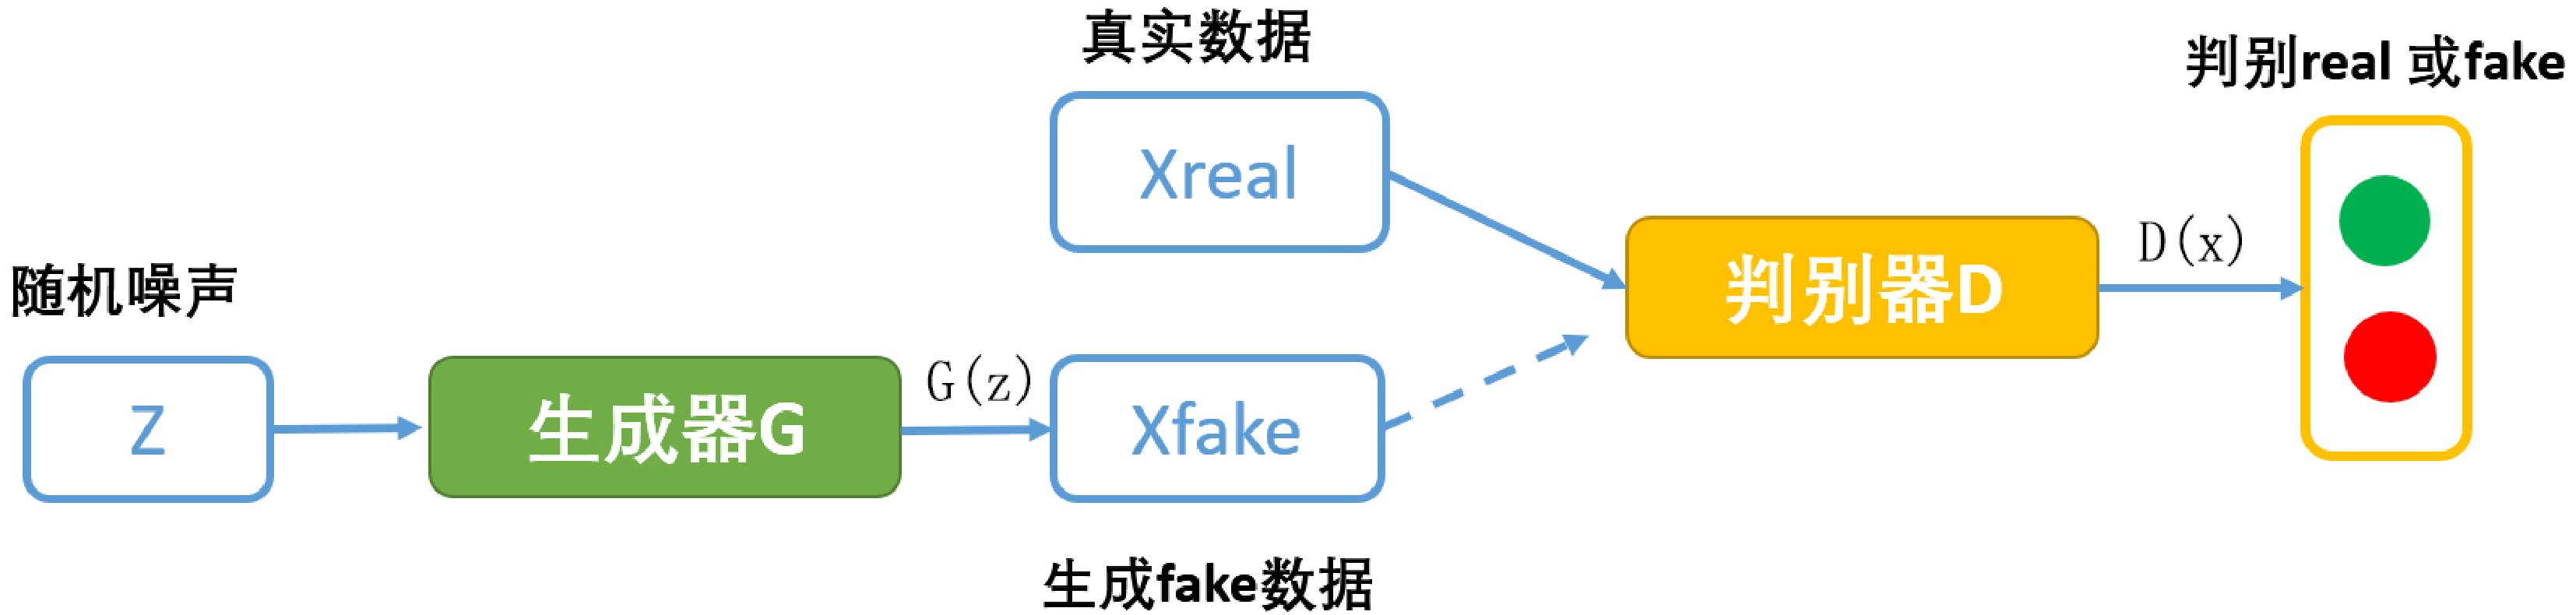
\includegraphics[width=0.8\textwidth]{figures/gan}
  \caption{GAN结构示意图}\label{fig:gan}
\end{figure}

如图\ref{fig:gan} 所示,假定变量$z$(通常为服从高斯分布的随机噪声)通过生成器G 生成$X_{fake}$,判别器D 负责判别输入的data 是生成的样本$X_{fake}$ 还是真实样本$X_{real}$。GAN 优化的目标函数为\ref{eq:4-1}:
\begin{equation}
  \label{eq:4-1}
  \mathop{\min}_{G} \mathop{\max}_{D} V(D,G) = \mathop{\min}_{G} \mathop{\max}_{D} E_{x \sim p_{data}(x)} [\log D(x)] + E_{z \sim p_{z}(z)}[ \log (1-D(G(z)))]
\end{equation}

式中$x \sim p_{data}(x)$ 表示$x$ 取自真实的分布数据。对于判别器D 来说,这是一个二分类问题,$ V(D,G)$ 为二分类中常见的交叉熵损失。对于生成器G 来说,为了尽可能欺骗D,需要最大化生成样本的判别概率$D(G(z))$ ,即最小化$\log (1-D(G(z)))$ 。

实际训练时,生成器G 和判别器D 采取交替训练,即先训练D ,再训练G ,不断往复。对于生成器G,最小化$\mathop{\max}_{D} V(D,G) $,即最小化$V(D,G)$ 的最大值。当生成器G 固定时,对$V(D,G)$ 求导,求出最优的判别器$D^{\star}(x)$:

\begin{equation}
  \label{eq:4-2}
  D^{\star}(x) = \frac{p_g(x)}{p_g(x)+p_{data}(x)}
\end{equation}

文献\cite{goodfellow2014generative} 中指出,当多次往复训练后,模型会收敛,G 与D 达到纳什均衡,此时$p_g(x) = p_{data}(x)$,即判别器对生成样本和真实样本的预测概率均为$\frac{1}{2}$, 无法区分。

传统的GAN 结构是无监督模型,只能生成真实的数据,不能生成我们想要的某一种类型的数据。文献\cite{mirza2014conditional} 提出条件生成对抗网络(Conditional Generative Adversarial Networks,CGAN),模型中加入条件约束$y$ 引导模型训练,生成我们需要的目标类型数据,$y$ 可以是任何种类的辅助信息,如样本标签,图像ground truth 图或其他不同领域模态的数据等。

\begin{figure}[htb]
  \centering
  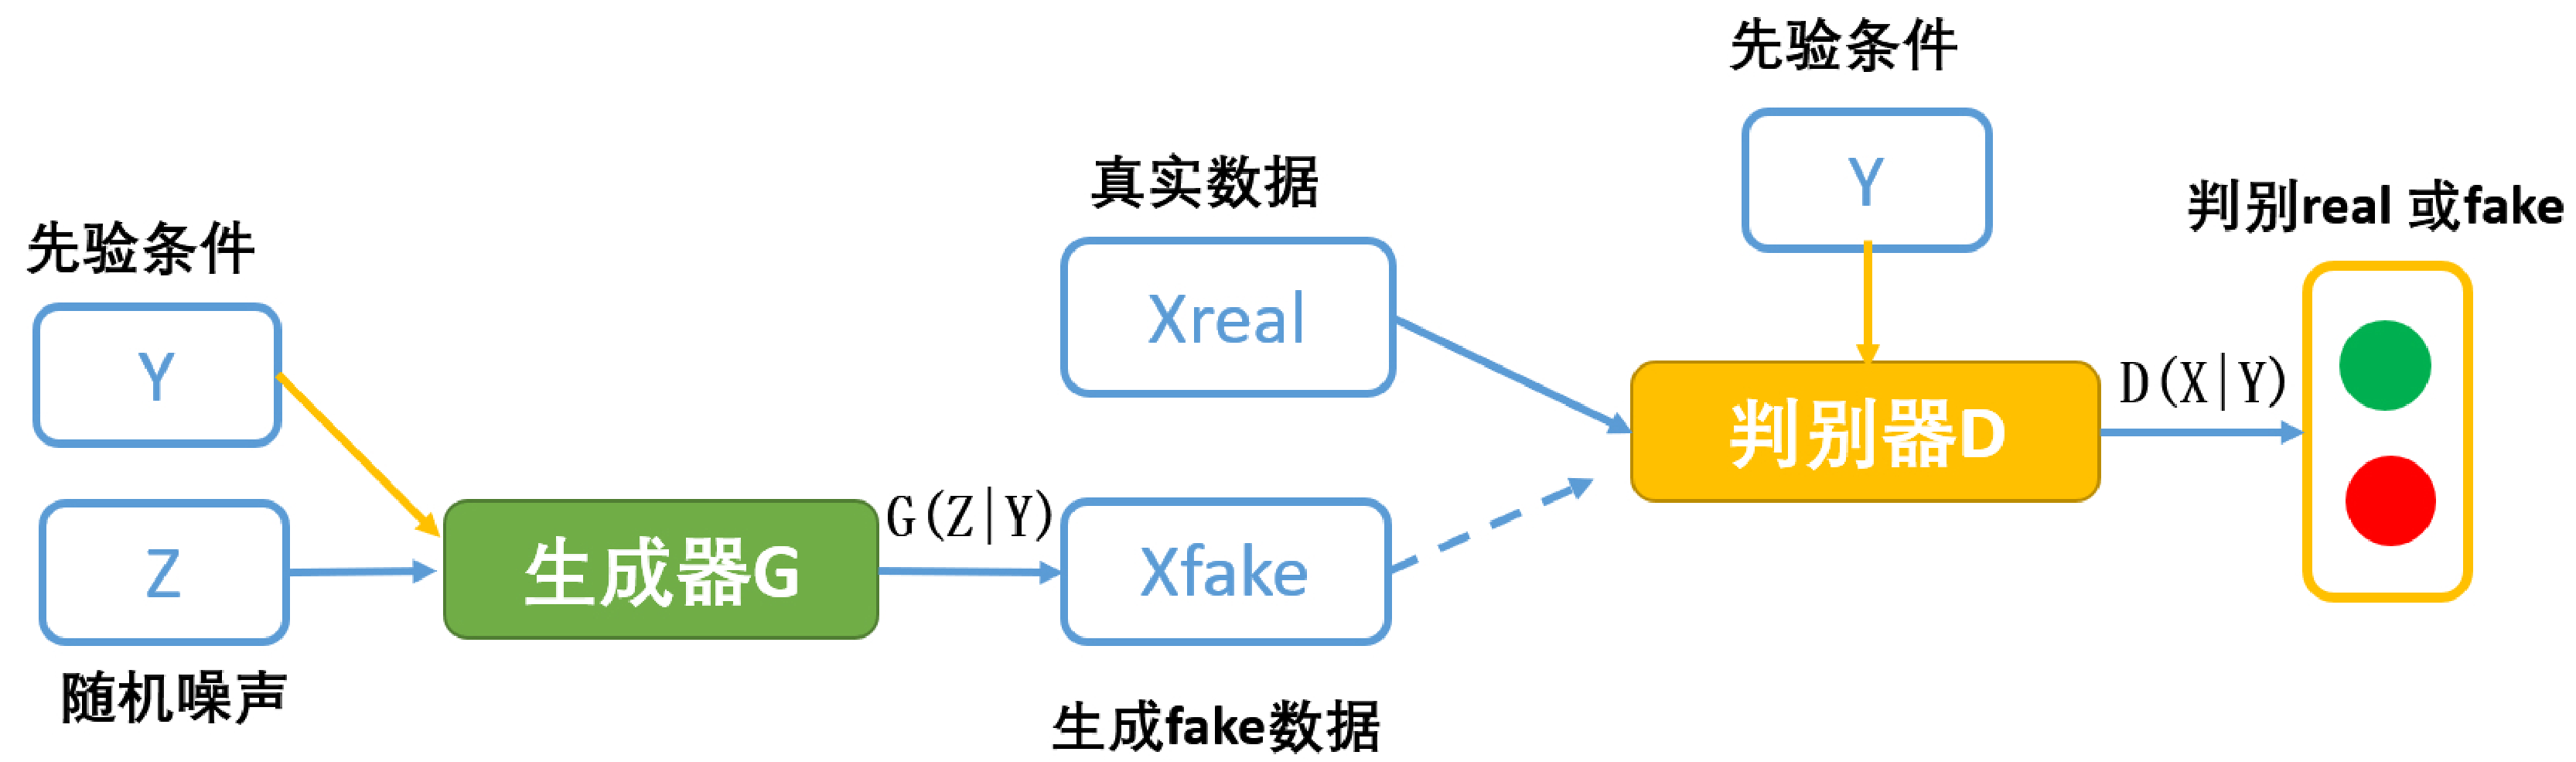
\includegraphics[width=0.8\textwidth]{figures/cgan}
  \caption{CGAN结构示意图}\label{fig:cgan}
\end{figure}

CGAN 模型中,生成器G 中随机噪声$z$与条件先验知识$y$ 被联合组成联合隐层输入特征;判别器D 中$X$ 和$y$ 通过词嵌入共同作为模型输入。 类似式\ref{eq:4-1}, CGAN 模型目标函数为带有条件概率的二人极小极大值博弈函数,即:

\begin{equation}
  \label{eq:4-3}
  \mathop{\min}_{G} \mathop{\max}_{D} V(D,G) = \mathop{\min}_{G} \mathop{\max}_{D} E_{x \sim p_{data}(x)} [\log D(x|y)] + E_{z \sim p_{z}(z)}[ \log (1-D(G(z|y)))]
\end{equation}

图\ref{fig:cgan} 为CGAN 的结构示意图,通过将额外条件信息$y$ 分别输送给判别模型和生成模型组成联合隐层表征,作为输入层的一部分,从而指导数据的生成过程。


\subsection{基于CGAN 的影像分割方法}
\label{sec:first-2}
基于图像条件的CGAN 影像分割方法主要包含两个阶段:生成网络的影像分割模型和对抗训练阶段的判别模型。整个方法处理流程如图\ref{fig:gan-fcn} 所示,左边生成网络是一个全卷积影像分割模型,右边对抗网络是一个二元分类判别模型。

\begin{figure}[htb]
  \centering
  \begin{center}
    \makebox[\textwidth]{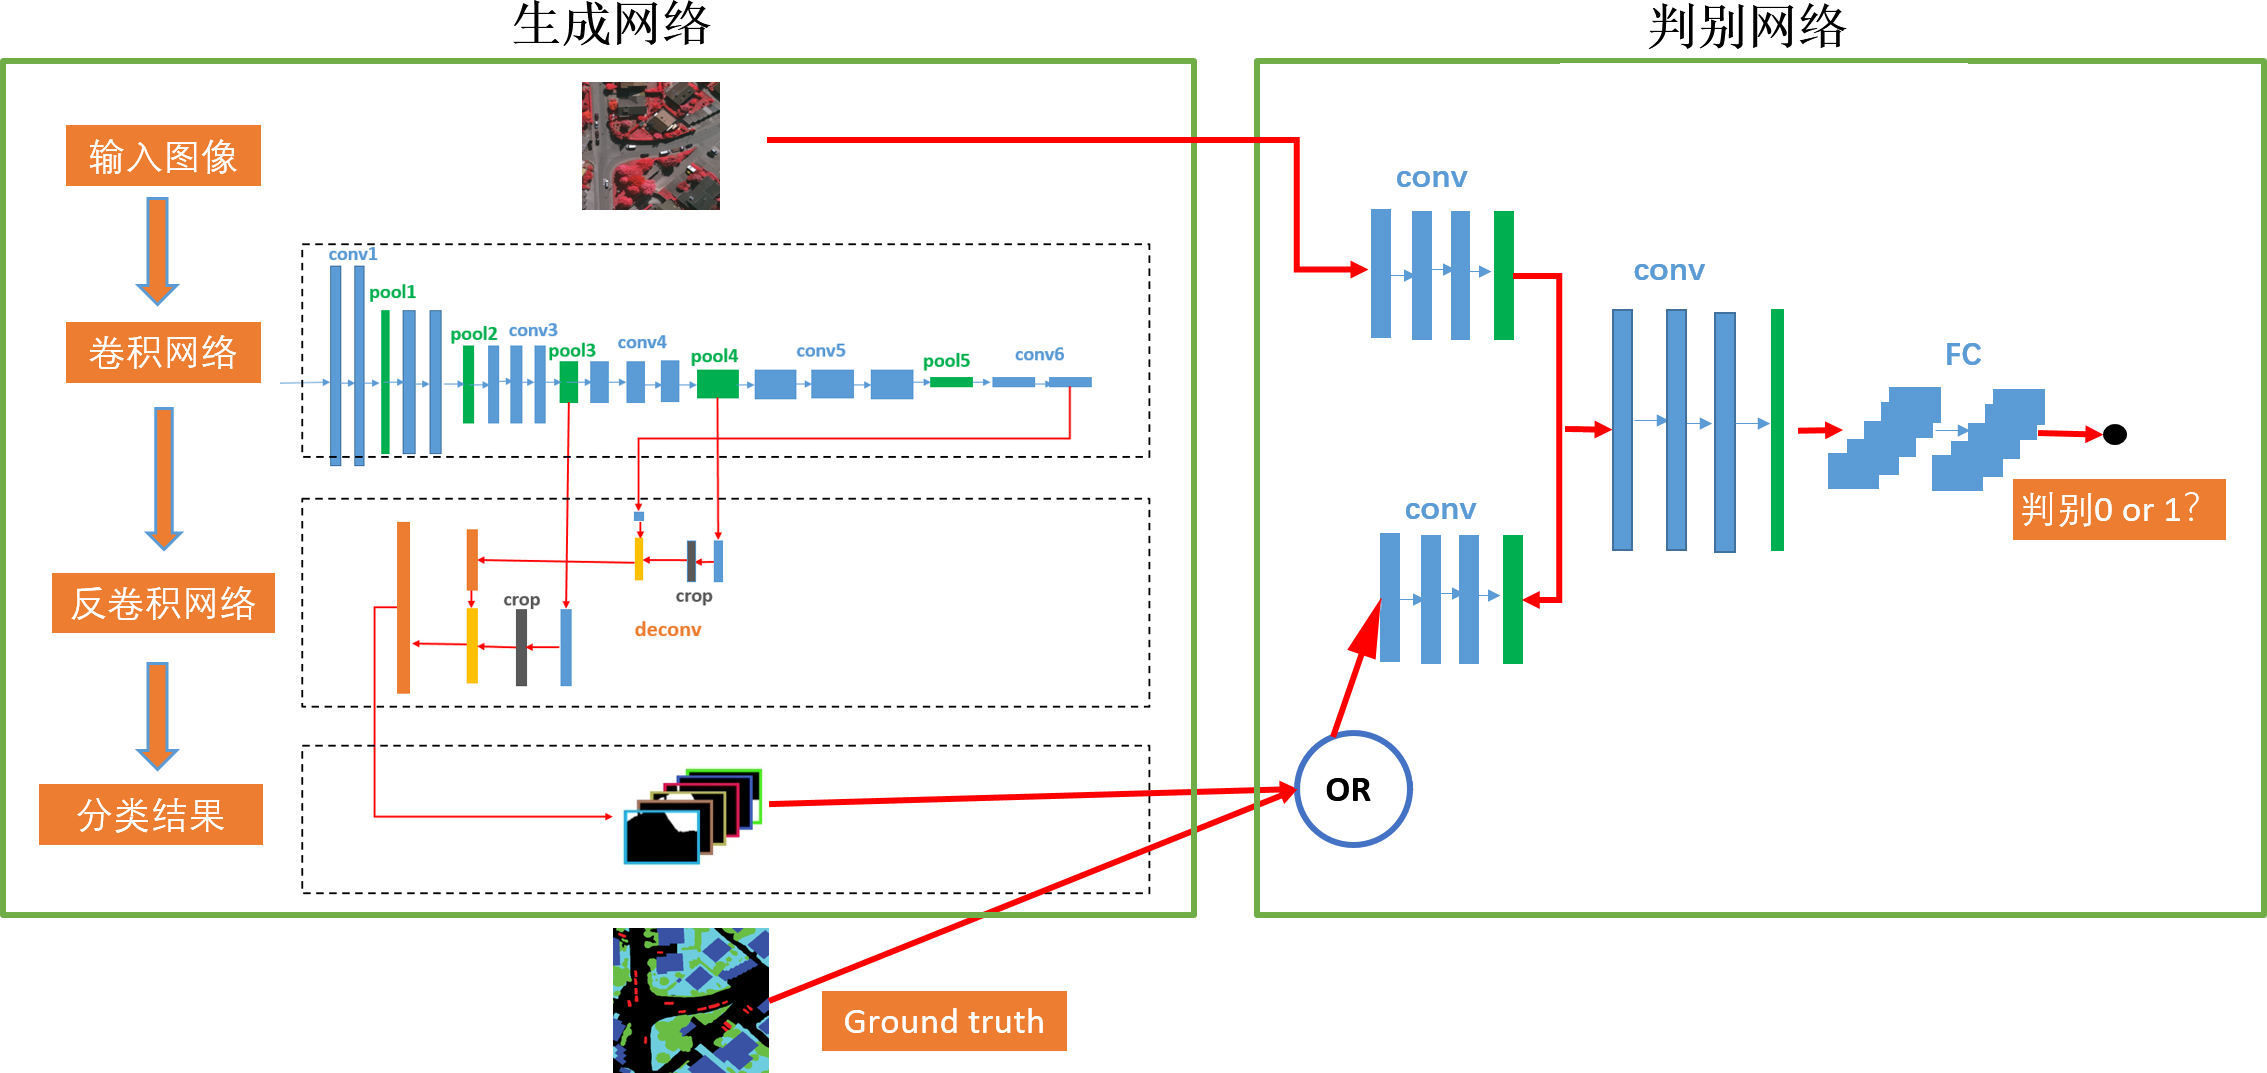
\includegraphics[width=\paperwidth]{figures/gan-fcn}}
    \caption{基于对抗训练框架的全卷积语义分割模型示意图}\label{fig:gan-fcn}
  \end{center}
\end{figure}

对抗网络的输入存在两种情况:一种是原始图像和ground truth 图拼接输入,另一种是原始图像与左边模型输出分割结果拼接输入。本文中对抗网络模型为一个六层卷积神经网络模型,一个卷积块由三个卷积层后接一个最大池化层组成,整个卷积网络由两个卷积块和两个全连接层堆叠形成。对抗网络的输出为一个二元分类值(输出为1代表它判断输入是第一种情况,输出为0代表它判断输入是第二种情况)。使用二元分类损失(Binary classification loss, BCE)来度量判别网络。二元分类损失为二元交叉熵(cross entropy)函数,统计学中使用KL 散度衡量两个事件或分布中的不同,常用于计算代价,而在特定任务下最小化KL散度等价于最小化交叉熵,而交叉熵的运算更简单\cite{de2005tutorial},所以这里用交叉熵来计算二元分类损失。交叉熵函数为分类预测概率值的负对数。二元交叉熵代价表达式如下:
\begin{equation}
  \label{eq:4-4}
  l_{bce} (\hat{z}, z) = -[z\log\hat{z} + (1-z)\log(1-\hat{z})]
\end{equation}
生成网络是全卷积网络模型,其是一个多分类网络模型。经典的多分类分割模型代价函数为多类别的交叉熵损失(multi-class entropy loss, MCE),则分割模型输入为大小为$H\times W\times C$ 的图像,对图像做像素级预测分类,其多元交叉熵损失为:
\begin{equation}
  \label{eq:4-5}
  l_{mce} (\hat{y}, y) = -\sum_{i=1}^{H\times W}\sum_{c=1}^{C}[y_{ic}\log\hat{y}_{ic} + (1-y_{ic})\log(1-\hat{y}_{ic})]
\end{equation}
其中,$H$、$W$ 和$C$ 分别为图像的高度、宽度以及通道数。对于使用独热编码(One-hot encode)将图像像素标签编码,其有$C$ 个标签类别,

对于有$N$ 张训练图片的数据集$X = \{x_1,x_2,\cdots, x_n \}$,其对应的ground truth 图标签集为$Y = \{y_1,y_2,\cdots, y_n \}$。

\section{实验数据介绍}
数据集

\section{实验结果与分析}
balabala

\section{本章小结}
balabala
%% !Mode:: "TeX:UTF-8"
%%% Local Variables:
%%% mode: latex
%%% TeX-master: t
%%% End:

\chapter{总结与展望}
\label{cha:chap05}

\section{本文的主要内容}
\label{sec:5-1}
遥感影像地物分类是遥感研究领域内一个重要问题,如何对地物类别正确识别、明确不同地物边界问题一直是一个研究热点。本文从正确预测地物边界、同类地物区域内像素保持空间一致性两个角度提出了现有高分影像地物分类方法的改进方法,且对提出的方法分别进行理论推导和实验论证。为了增强影像分割像素点间的连续性,文中将对抗训练的思想应用到FCN 分类模型中,提出了基于CGAN 影像分类方法。针对遥感影像混淆边界与模型中边界信息的损失问题,文中提出融合边界特征信息的CGAN 影像分类方法。针对影像分类中细碎区域的错分问题,文中提出基于辅助信息后处理的CGAN 影像分类方法。具体研究工作如下:
\begin{enumerate}[(1)]
  \item 针对全卷积分割方法中上采样特征损失的问题,文中将对抗训练网络思想应用到FCN 模型中,提出基于CGAN 的全卷积影像分类方法,提升影像分类效果。融合影像正射影像波段和DSM 高程波段数据用于模型训练。在Vaihingen 影像数据上的实验结果表明基于CGAN 的影像分类方法能够获得更好的分类效果。
  \item 针对因生成网络中池化操作和上采样操作导致的影像边界、位置信息损失的问题。首先由TFSV-IT2FCM 方法预处理得到影像分割单元边界图,然后在生成模型上采样操作的特征图内融合相同尺度的边界掩膜特征信息,提升高阶语义特征的边界位置信息,提出了融合边界特征的 CGAN 影像分类方法。实验结果表明融合边界特征的CGAN 影像分类方法能够获得更明确的地物分类边界。
  \item 针对生成模型中各像素点未考虑邻近像素点间的关系,从而导致复杂地物类别出现错分区域的问题。文中考虑像素点所属同质性分割单元内其他像素点的类别预测关系,优化像素点类别预测概率,提出了基于辅助信息后处理的影像分类方法。添加后处理的方法在Vaihingen 数据集上的结果提升了同类地物区域内像素点的空间一致性。
  \item 将融合边界特征和辅助信息后处理两种改进思路同时引入基于CGAN 影像分类方法中,改进影像分类的效果,实验结果证明了这两种方法的有效性。
\end{enumerate}


\section{未来的期望}
\label{sec:5-2}
本文提出的影像分类的改进方法,一定程度上均能提升遥感影像地物分类边界划分的效果,同时也能提高同类别地物区域像素点的空间一致性。之后的研究可从以下方面开展:
\begin{enumerate}[(1)]
  \item  第~\ref{cha:chap03} 章提出的基于CGAN 影像分类方法在识别“车辆”时相对其他几类地物精度较低,原因是训练集影像中含有“车辆”的像素点占比较低,后续研究中构建模型目标函数时可以考虑给像素占比低的地物一个较高的权值,研究加权后的交叉熵代价能否提高像素占比小地物的识别效果。
  \item  第\ref{cha:chap04} 章融合边界特征方法中,融合边界掩膜时采取矩阵点乘的操作进行特征融合,其他方式的特征融合方法可以进一步研究探讨。
  \item  第\ref{cha:chap04} 章基于辅助信息后处理的方法中只考虑像素点同质性分割单元内其他像素点的类别预测概率。后续研究可以考虑整幅影像中所有像素点之间的相互关系,对该像素点类别预测概率进行处理、优化。
  
\end{enumerate}
% !Mode:: "TeX:UTF-8"
%%% Local Variables:
%%% mode: latex
%%% TeX-master: t
%%% End:

\chapter{总结与展望}
\label{cha:chap06}



小老鼠偷吃热凉粉;短长虫环绕矮高粱。\footnote{韩愈(768-824),字退之,河南河阳(
  今河南孟县)人,自称郡望昌黎,世称韩昌黎。幼孤贫刻苦好学,德宗贞元八年进士。曾
  任监察御史,因上疏请免关中赋役,贬为阳山县令。后随宰相裴度平定淮西迁刑部侍郎,
  又因上表谏迎佛骨,贬潮州刺史。做过吏部侍郎,死谥文公,故世称韩吏部、韩文公。是
  唐代古文运动领袖,与柳宗元合称韩柳。诗力求险怪新奇,雄浑重气势。}


\section{本文的主要内容}
封面的例子请参看 cover.tex。主要符号表参看 denation.tex,附录和个人简历分别参看 appendix01.tex
和 resume.tex。里面的命令都非常简单,一看即会。\footnote{你说还是看不懂?怎么会呢?}

\section{未来的期望}
\label{sec:first}

苏轼(1037-1101),北宋文学家、书画家。字子瞻,号东坡居士,眉州眉山(今属四川)人




%%% 其它部分
%\backmatter



% % 参考文献
\bibliographystyle{bnubib}
\bibliography{ref/refs}

% 致谢
% !Mode:: "TeX:UTF-8"
%%% Local Variables:
%%% mode: latex
%%% TeX-master: "../main"
%%% End:

\begin{ack}
  快乐的时间总是过得很快,转瞬之间,我在北京师范大学三年的硕士研究生生活即将结束。离别之际,我要向帮助和关照我的老师、家人、同学和好友们表示感谢,谢谢你们!

  首先感谢我的两位指导老师:余先川教授和胡丹副教授。还记得三年前刚来北京师范大学学习的时候,我对实验室研究工作和科研方向都比较迷茫,是胡丹老师指导我开展科研学习的工作,是胡老师告诉我如何去看论文,怎样学习研究学者思考问题的方式。每周一到两次的讨论中胡老师也时常跟我探讨课题中的知识,对于我的困惑与科研中遇到的问题,胡老师都耐心的和我沟通、讨论。研二下学期伊始,胡丹老师去美国从事新的事业,虽然远隔重洋,但还时常接收到胡老师来自大洋彼岸的关心和问候。同时胡老师在生活上对我也非常热心,有时候生活上不如意或遇到烦心事,胡老师也体贴入微,关心并疏导我的个人问题,感谢胡老师近两年对我学习和生活上的关怀。胡老师出国后,我转到现在的导师余先川教授下继续从事科研学习。我也由衷地感谢余老师,余老师在专业学科领域有极其敏锐的洞察力,能够迅速了解当前领域内研究的前沿内容。在余老师的指导下,我能够在遥感影像数据挖掘领域继续深入研究,提升自己的科研能力。毕业论文从开题到撰写过程中,余老师都认真、耐心地指导我并指出论文中存在的问题与不足。在生活上,余老师待人亲切,关心学生,更像是实验室大家庭的家长,实验室经常性的聚餐、实验室每个小伙伴生日会的庆祝与祝福都让远离家乡,漂泊北京的我们感受到了来自家庭的温暖。此外,余老师也会带着我们去参加一些前沿学术论坛和会议,让我们接触到学术界的科研大牛的同时,也开阔拓展了我们的视野。再次对我两位导师表示致谢!

  其次感谢实验室的张立保老师,张老师严谨的科研态度值得我学习,另外感谢张老师在电子楼512室给我提供的科研工位,让我更便利地从事科研学习。同时感谢师母的关照,感谢师母对实验室学生的关心和支持,师母也让我们体会到慈爱家长般的温暖。

  感谢实验室的每一位同学,和大家在一起学习、生活的时光让我快乐、开心,感谢实验室里每一位师兄师姐师弟和师妹们。

  感谢我的室友冯思博、朱云宗和戎博杰,谢谢你们三年的陪伴,大家一起度过的研究生时光也会成为我心中的美好记忆。

  最后,我要感谢我的父母亲人们对我的关怀和照顾。你们在我背后默默的奉献与付出,一直是我坚持前行的动力,是你们在我迷茫的时候给我支持和力量,鼓励我面对困难,笑对困难与挫折。

  漫漫人生路,几度欢乐,几度忧愁,正因此才能体会到生命与生活的多彩。未来的路还很漫长,心怀感恩砥砺前行。

\end{ack}


% 附录
%\begin{appendix}
%% !Mode:: "TeX:UTF-8"
%%% Local Variables: 
%%% mode: latex
%%% TeX-master: "../main"
%%% End: 

\chapter{外文资料原文}
\label{cha:engorg}
As one of the most widely used techniques in operations research, {\em
  mathematical programming} is defined as a means of maximizing a quantity known
as {\em objective function}, subject to a set of constraints represented by
equations and inequalities. Some known subtopics of mathematical programming are
linear programming, nonlinear programming, multiobjective programming, goal
programming, dynamic programming, and multilevel programming$^{[1]}$.

It is impossible to cover in a single chapter every concept of mathematical
programming. This chapter introduces only the basic concepts and techniques of
mathematical programming such that readers gain an understanding of them
throughout the book$^{[2,3]}$.


\section{Single-Objective Programming}
The general form of single-objective programming (SOP) is written
as follows,
\begin{equation}\tag*{(123)} % 如果附录中的公式不想让它出现在公式索引中,那就请
                             % 用 \tag*{xxxx}
\left\{\begin{array}{l}
\max \,\,f(x)\\[0.1 cm]
\mbox{subject to:} \\ [0.1 cm]
\qquad g_j(x)\le 0,\quad j=1,2,\cdots,p
\end{array}\right.
\end{equation}
which maximizes a real-valued function $f$ of
$x=(x_1,x_2,\cdots,x_n)$ subject to a set of constraints.

\newtheorem{mpdef}{Definition}[chapter]
\begin{mpdef}
In SOP, we call $x$ a decision vector, and
$x_1,x_2,\cdots,x_n$ decision variables. The function
$f$ is called the objective function. The set
\begin{equation}\tag*{(456)} % 这里同理,其它不再一一指定。
S=\left\{x\in\Re^n\bigm|g_j(x)\le 0,\,j=1,2,\cdots,p\right\}
\end{equation}
is called the feasible set. An element $x$ in $S$ is called a
feasible solution.
\end{mpdef}

\newtheorem{mpdefop}[mpdef]{Definition}
\begin{mpdefop}
A feasible solution $x^*$ is called the optimal
solution of SOP if and only if
\begin{equation}
f(x^*)\ge f(x)
\end{equation}
for any feasible solution $x$.
\end{mpdefop}

One of the outstanding contributions to mathematical programming was known as
the Kuhn-Tucker conditions\ref{eq:ktc}. In order to introduce them, let us give
some definitions. An inequality constraint $g_j(x)\le 0$ is said to be active at
a point $x^*$ if $g_j(x^*)=0$. A point $x^*$ satisfying $g_j(x^*)\le 0$ is said
to be regular if the gradient vectors $\nabla g_j(x)$ of all active constraints
are linearly independent.

Let $x^*$ be a regular point of the constraints of SOP and assume that all the
functions $f(x)$ and $g_j(x),j=1,2,\cdots,p$ are differentiable. If $x^*$ is a
local optimal solution, then there exist Lagrange multipliers
$\lambda_j,j=1,2,\cdots,p$ such that the following Kuhn-Tucker conditions hold,
\begin{equation}
\label{eq:ktc}
\left\{\begin{array}{l}
    \nabla f(x^*)-\sum\limits_{j=1}^p\lambda_j\nabla g_j(x^*)=0\\[0.3cm]
    \lambda_jg_j(x^*)=0,\quad j=1,2,\cdots,p\\[0.2cm]
    \lambda_j\ge 0,\quad j=1,2,\cdots,p.
\end{array}\right.
\end{equation}
If all the functions $f(x)$ and $g_j(x),j=1,2,\cdots,p$ are convex and
differentiable, and the point $x^*$ satisfies the Kuhn-Tucker conditions
(\ref{eq:ktc}), then it has been proved that the point $x^*$ is a global optimal
solution of SOP.

\subsection{Linear Programming} 
\label{sec:lp}

If the functions $f(x),g_j(x),j=1,2,\cdots,p$ are all linear, then SOP is called
a {\em linear programming}.

The feasible set of linear is always convex. A point $x$ is called an extreme
point of convex set $S$ if $x\in S$ and $x$ cannot be expressed as a convex
combination of two points in $S$. It has been shown that the optimal solution to
linear programming corresponds to an extreme point of its feasible set provided
that the feasible set $S$ is bounded. This fact is the basis of the {\em simplex
  algorithm} which was developed by Dantzig as a very efficient method for
solving linear programming.
\begin{table}[ht]
\centering
  \centering
  \caption*{Table~1\hskip1em This is an example for manually numbered table, which would not appear in the list of tables}
  \label{tab:badtabular2}
  \begin{tabular}[c]{|c|m{0.8in}|c|c|c|c|c|}\hline
    \multicolumn{2}{|c|}{Network Topology} & \# of nodes & 
    \multicolumn{3}{c|}{\# of clients} & Server \\\hline
    GT-ITM & Waxman Transit-Stub & 600 &
    \multirow{2}{2em}{2\%}& 
    \multirow{2}{2em}{10\%}& 
    \multirow{2}{2em}{50\%}& 
    \multirow{2}{1.2in}{Max. Connectivity}\\\cline{1-3}
    \multicolumn{2}{|c|}{Inet-2.1} & 6000 & & & &\\\hline
    \multirow{2}{1in}{Xue} & Rui  & Ni &\multicolumn{4}{c|}{\multirow{2}*{\bnuthesis}}\\\cline{2-3}
    & \multicolumn{2}{c|}{ABCDEF} &\multicolumn{4}{c|}{} \\\hline
\end{tabular}  
\end{table}

Roughly speaking, the simplex algorithm examines only the extreme points of the
feasible set, rather than all feasible points. At first, the simplex algorithm
selects an extreme point as the initial point. The successive extreme point is
selected so as to improve the objective function value. The procedure is
repeated until no improvement in objective function value can be made. The last
extreme point is the optimal solution.

\subsection{Nonlinear Programming}

If at least one of the functions $f(x),g_j(x),j=1,2,\cdots,p$ is nonlinear, then
SOP is called a {\em nonlinear programming}.

A large number of classical optimization methods have been developed to treat
special-structural nonlinear programming based on the mathematical theory
concerned with analyzing the structure of problems.

Now we consider a nonlinear programming which is confronted solely with
maximizing a real-valued function with domain $\Re^n$.  Whether derivatives are
available or not, the usual strategy is first to select a point in $\Re^n$ which
is thought to be the most likely place where the maximum exists. If there is no
information available on which to base such a selection, a point is chosen at
random. From this first point an attempt is made to construct a sequence of
points, each of which yields an improved objective function value over its
predecessor. The next point to be added to the sequence is chosen by analyzing
the behavior of the function at the previous points. This construction continues
until some termination criterion is met. Methods based upon this strategy are
called {\em ascent methods}, which can be classified as {\em direct methods},
{\em gradient methods}, and {\em Hessian methods} according to the information
about the behavior of objective function $f$. Direct methods require only that
the function can be evaluated at each point. Gradient methods require the
evaluation of first derivatives of $f$. Hessian methods require the evaluation
of second derivatives. In fact, there is no superior method for all
problems. The efficiency of a method is very much dependent upon the objective
function.


\chapter{外文资料的调研阅读报告或书面翻译}
\section{单目标规划}
北冥有鱼,其名为鲲。鲲之大,不知其几千里也。化而为鸟,其名为鹏。鹏之背,不知其几
千里也。怒而飞,其翼若垂天之云。是鸟也,海运则将徙于南冥。南冥者,天池也。 
\begin{equation}\tag*{(123)}
 p(y|\mathbf{x}) = \frac{p(\mathbf{x},y)}{p(\mathbf{x})}=
\frac{p(\mathbf{x}|y)p(y)}{p(\mathbf{x})}
\end{equation}

吾生也有涯,而知也无涯。以有涯随无涯,殆已!已而为知者,殆而已矣!为善无近名,为
恶无近刑,缘督以为经,可以保身,可以全生,可以养亲,可以尽年。

\subsection{线性规划}
庖丁为文惠君解牛,手之所触,肩之所倚,足之所履,膝之所倚,砉然响然,奏刀騞然,莫
不中音,合于桑林之舞,乃中经首之会。
\begin{table}[ht]
\centering
  \caption*{表~A1\hskip1em 这是手动编号但不出现在索引中的一个表格例子}
  \label{tab:badtabular3}
  \begin{tabular}[c]{|c|m{0.8in}|c|c|c|c|c|}\hline
    \multicolumn{2}{|c|}{Network Topology} & \# of nodes & 
    \multicolumn{3}{c|}{\# of clients} & Server \\\hline
    GT-ITM & Waxman Transit-Stub & 600 &
    \multirow{2}{2em}{2\%}& 
    \multirow{2}{2em}{10\%}& 
    \multirow{2}{2em}{50\%}& 
    \multirow{2}{1.2in}{Max. Connectivity}\\\cline{1-3}
    \multicolumn{2}{|c|}{Inet-2.1} & 6000 & & & &\\\hline
    \multirow{2}{1in}{Xue} & Rui  & Ni &\multicolumn{4}{c|}{\multirow{2}*{\bnuthesis}}\\\cline{2-3}
    & \multicolumn{2}{c|}{ABCDEF} &\multicolumn{4}{c|}{} \\\hline
\end{tabular}  
\end{table}

\begin{table}[ht]
\centering
  \caption{正常附录表格的例子}
  \label{tab:badtabular3}
  \begin{tabular}[c]{|c|m{0.8in}|c|c|c|c|c|}\hline
    \multicolumn{2}{|c|}{Network Topology} & \# of nodes & 
    \multicolumn{3}{c|}{\# of clients} & Server \\\hline
    GT-ITM & Waxman Transit-Stub & 600 &
    \multirow{2}{2em}{2\%}& 
    \multirow{2}{2em}{10\%}& 
    \multirow{2}{2em}{50\%}& 
    \multirow{2}{1.2in}{Max. Connectivity}\\\cline{1-3}
    \multicolumn{2}{|c|}{Inet-2.1} & 6000 & & & &\\\hline
    \multirow{2}{1in}{Xue} & Rui  & Ni &\multicolumn{4}{c|}{\multirow{2}*{\bnuthesis}}\\\cline{2-3}
    & \multicolumn{2}{c|}{ABCDEF} &\multicolumn{4}{c|}{} \\\hline
\end{tabular}  
\end{table}

文惠君曰:“嘻,善哉!技盖至此乎?”庖丁释刀对曰:“臣之所好者道也,进乎技矣。始臣之
解牛之时,所见无非全牛者;三年之后,未尝见全牛也;方今之时,臣以神遇而不以目视,
官知止而神欲行。依乎天理,批大郤,导大窾,因其固然。技经肯綮之未尝,而况大坬乎!
良庖岁更刀,割也;族庖月更刀,折也;今臣之刀十九年矣,所解数千牛矣,而刀刃若新发
于硎。彼节者有间而刀刃者无厚,以无厚入有间,恢恢乎其于游刃必有余地矣。是以十九年
而刀刃若新发于硎。虽然,每至于族,吾见其难为,怵然为戒,视为止,行为迟,动刀甚微,
謋然已解,如土委地。提刀而立,为之而四顾,为之踌躇满志,善刀而藏之。”

文惠君曰:“善哉!吾闻庖丁之言,得养生焉。”


\subsection{非线性规划}
孔子与柳下季为友,柳下季之弟名曰盗跖。盗跖从卒九千人,横行天下,侵暴诸侯。穴室枢
户,驱人牛马,取人妇女。贪得忘亲,不顾父母兄弟,不祭先祖。所过之邑,大国守城,小
国入保,万民苦之。孔子谓柳下季曰:“夫为人父者,必能诏其子;为人兄者,必能教其弟。
若父不能诏其子,兄不能教其弟,则无贵父子兄弟之亲矣。今先生,世之才士也,弟为盗
跖,为天下害,而弗能教也,丘窃为先生羞之。丘请为先生往说之。”

柳下季曰:“先生言为人父者必能诏其子,为人兄者必能教其弟,若子不听父之诏,弟不受
兄之教,虽今先生之辩,将奈之何哉?且跖之为人也,心如涌泉,意如飘风,强足以距敌,
辩足以饰非。顺其心则喜,逆其心则怒,易辱人以言。先生必无往。”

孔子不听,颜回为驭,子贡为右,往见盗跖。


\chapter{其它附录}
前面两个附录主要是给本科生做例子。其它附录的内容可以放到这里,当然如果你愿意,可
以把这部分也放到独立的文件中,然后将其 \verb|\input| 到主文件中。
%\end{appendix}
%
% % 学术成果
% !Mode:: "TeX:UTF-8"
\begin{paper}
\begin{enumerate}
  \item \textbf{Tao Jiang}, Dan Hu, and Xianchuan Yu.  Enhanced IT2FCM algorithm using object-based triangular fuzzy set modeling for remote-sensing clustering[J]. Computers \& geosciences, 2018, 118: 14-26. (SCI 三区收录, 检索号:GQ6TC.)
  \item Dan Hu, \textbf{Tao Jiang}, and Xianchuan Yu. The construction of non-convex fuzzy sets. 2017 13th ICNC-FSKD, Guilin, 2017, pp. 1175-1181. (EI 收录, 检索号:20183005590187.)
  \item Haihua Xing, Hui He, Xianchuan Yu, Dan Hu, \textbf{Tao Jiang}.  An Interval Type-2 Fuzzy Sets Generation Method for Remote Sensing Imagery Classification[J]. Computers \& geosciences, 2019.(SCI 三区, accept)\\

  \end{enumerate}

\end{paper}

%International Conference on Natural Computation, Fuzzy Systems and Knowledge  Discovery ()

% \hspace*{6em}



\begin{center}
  \large {\hei 研究生期间主要参与项目 }
\end{center}

\begin{enumerate}[(1)]
\item 自适应循优 $n$ 型模糊系统及其应用研究, 国家自然科学基金面上项目(11471045),2015.01-2018.12.

\item 基于深度学习的遥感崩滑地质灾害信息提取,北京市自然科学基金(L172029),2017.10-
2019.12.\\

\end{enumerate}





\end{document}
